\documentclass[11pt]{article}

\usepackage[margin=1in]{geometry}
\usepackage{amsmath,amssymb,amsfonts,amsthm,bm,mathtools,mathrsfs}
\usepackage{booktabs}
\usepackage{graphicx}
\usepackage{enumitem}
\usepackage{algorithm}
\usepackage{algpseudocode}
\usepackage{xcolor}
\usepackage{natbib}
\usepackage{tikz}
\usetikzlibrary{arrows.meta,positioning,calc,fit,shapes.geometric}
\usepackage[colorlinks=true,linkcolor=blue,citecolor=blue,urlcolor=blue]{hyperref}

\graphicspath{{experiments/causal_atlas_bridge/figures/}}

\numberwithin{equation}{section}
\newtheorem{assumption}{Assumption}[section]
\newtheorem{condition}{Condition}[section]
\newtheorem{definition}{Definition}[section]
\newtheorem{theorem}{Theorem}[section]
\newtheorem{lemma}{Lemma}[section]
\newtheorem{proposition}{Proposition}[section]
\newtheorem{corollary}{Corollary}[section]
\newtheorem{example}{Example}[section]
\newtheorem{remark}{Remark}[section]

\DeclareMathOperator{\Var}{Var}
\DeclareMathOperator{\Cov}{Cov}
\DeclareMathOperator{\rank}{rank}
\DeclareMathOperator{\diam}{diam}
\DeclareMathOperator{\sign}{sign}
\DeclareMathOperator{\dist}{dist}
\DeclareMathOperator{\conv}{conv}
\DeclareMathOperator{\cl}{cl}
\DeclareMathOperator{\supp}{supp}
\DeclareMathOperator{\Unif}{Unif}
\DeclareMathOperator*{\argmin}{arg\,min}
\DeclareMathOperator*{\argmax}{arg\,max}

\newcommand{\E}{\mathbb E}
\newcommand{\Pbb}{\mathbb P}
\newcommand{\R}{\mathbb R}
\newcommand{\N}{\mathbb N}
\newcommand{\1}{\mathbf 1}
\newcommand{\cA}{\mathcal A}
\newcommand{\cB}{\mathcal B}
\newcommand{\cC}{\mathcal C}
\newcommand{\cD}{\mathcal D}
\newcommand{\cE}{\mathcal E}
\newcommand{\cF}{\mathcal F}
\newcommand{\cG}{\mathcal G}
\newcommand{\cH}{\mathcal H}
\newcommand{\cI}{\mathcal I}
\newcommand{\cJ}{\mathcal J}
\newcommand{\cK}{\mathcal K}
\newcommand{\cL}{\mathcal L}
\newcommand{\cM}{\mathcal M}
\newcommand{\cN}{\mathcal N}
\newcommand{\cO}{\mathcal O}
\newcommand{\cP}{\mathcal P}
\newcommand{\cQ}{\mathcal Q}
\newcommand{\cR}{\mathcal R}
\newcommand{\cS}{\mathcal S}
\newcommand{\cT}{\mathcal T}
\newcommand{\cU}{\mathcal U}
\newcommand{\cV}{\mathcal V}
\newcommand{\cW}{\mathcal W}
\newcommand{\cX}{\mathcal X}
\newcommand{\cY}{\mathcal Y}
\newcommand{\cZ}{\mathcal Z}
\newcommand{\norm}[1]{\left\lVert #1\right\rVert}
\newcommand{\abs}[1]{\left\lvert #1\right\rvert}
\newcommand{\ip}[2]{\left\langle #1,#2\right\rangle}
\newcommand{\defeq}{\vcentcolon=}
\newcommand{\eps}{\varepsilon}
\newcommand{\iid}{\overset{\mathrm{iid}}{\sim}}
\newcommand{\ind}{\perp\!\!\!\perp}
\newcommand{\given}{\,\middle|\,}
\newcommand{\Normal}{\mathsf N}
\newcommand{\Ber}{\mathsf{Bernoulli}}
\newcommand{\op}{o_{\Pbb}}
\newcommand{\Op}{O_{\Pbb}}
\newcommand{\br}{\operatorname{br}}
\newcommand{\poly}{\operatorname{poly}}
\newcommand{\calpha}{\alpha}
\tikzset{
  box/.style={draw, rounded corners=2pt, thick, align=center, minimum height=12mm, text width=3.3cm, inner sep=4pt, fill=gray!8},
  bluebox/.style={box, fill=blue!7},
  greenbox/.style={box, fill=green!8},
  purplebox/.style={box, fill=purple!8},
  orangebox/.style={box, fill=orange!12},
  redbox/.style={box, fill=red!7},
  arrow/.style={-Latex, thick},
  dashedarrow/.style={-Latex, thick, dashed}
}

\title{A Rejectable Causal Atlas for Experimental Archives:\ Composability, Honest Partial Identification, and Bridge Experiment Design}
\author{CAUSAL Lab Research Blueprint}
\date{}

\begin{document}
\maketitle

\begin{abstract}
Modern experimentation is no longer scarce.  Platform science, policy evaluation, and AI evaluation systems routinely produce archives containing many randomized or quasi-randomized contrasts, but these contrasts are usually stored as isolated point estimates.  This paper asks when such an archive can be upgraded into a \emph{causal atlas}: a structured map that composes old experiments only when their mechanisms, designs, and uncertainty certificates license transport to a target contrast; refuses composition when the archive lacks support; and selects bridge experiments that shrink the remaining unidentified region.  The key object is therefore not semantic similarity between study descriptions, but a rejectable certificate of causal composability.  We formalize each archive element as a treatment--outcome--context--design object endowed with an assumption profile, a mechanism representation, and an experiment-level debiased estimator.  Under local smoothness, design compatibility, support, and moderator-sensitivity conditions, we prove a finite-sample composition inequality whose terms separate causal support error, curvature, statistical noise, nuisance-debiasing error, and hidden-moderator residuals.  The construction retains the standard exact unbiasedness of Horvitz--Thompson/AIPW estimation under known randomization and carries its nuisance remainder and variance certificate into the atlas analysis.  We further establish asymptotic normality and honest confidence intervals for atlas compositions, an impossibility theorem showing that semantic proximity alone cannot certify transport under hidden moderators, a valid partial-identification construction after rejection, a minimax lower bound showing that unsupported targets cannot be estimated faster than the certified gap permits, and a weak-submodular guarantee for greedy bridge design.  Synthetic experiments with known mechanisms and a real-data NSW job-training local-contrast archive show that causal support improves reconstruction, restores interval coverage, and selects bridges that reduce unidentified regions more efficiently than semantic baselines.
\end{abstract}

\section{Introduction}
\label{sec:introduction}

Causal ATLAS is a research program for turning experimental archives, LLM-generated interventions, routing logs, and strategic AI deployments into an identifiable, composable, and decision-aware causal map.  This first paper supplies the archive-to-discovery layer of that program.  Its central question is deliberately prior to prediction: \emph{when is it mathematically legitimate to reuse one experiment as evidence about another?}

\paragraph{The broad field.}
Empirical science increasingly operates in an archival regime.  A large digital platform may run thousands of A/B tests; a policy area may contain decades of randomized field experiments; an AI laboratory may evaluate prompts, model-routing choices, safety interventions, and user-interface treatments under partially overlapping tasks.  The scientific promise is obvious: previous experiments should reduce the cost of new experimentation.  The statistical danger is equally obvious: experiments that look similar in text, share a high-level topic, or have nearby embeddings need not identify the same causal effect.  The broad field is therefore causal evidence synthesis: the attempt to combine randomized, quasi-randomized, and logged evidence without erasing the assumptions that made each piece of evidence credible.

\paragraph{The subproblem.}
Classical meta-analysis starts after a common estimand has been declared.  Transportability theory asks whether an effect can be moved from one environment to another under structural assumptions.  Representation-learning approaches retrieve studies by semantic or geometric proximity.  The present paper studies the layer between retrieval and aggregation.  Given an archive of experimental findings and a new target contrast, we ask whether the archive contains enough \emph{causal support} to identify, approximate, or honestly bound the target effect.  It is an identification problem over a finite and imperfect experimental archive.

\paragraph{A motivating failure.}
Consider a policy platform containing three apparently nearby interventions: a motivational email for job seekers, a peer-comparison message about job-search intensity, and a hiring-signal badge shown to employers.  A language model may place all three close to a proposed target intervention, because the descriptions share vocabulary about encouragement, salience, or social proof.  Yet their effects can depend on moderators not present in the text, such as baseline motivation or local labor-market tightness.  They may also differ in experiment design: the treatment contrast, control-condition intensity, measurement scale, timing, exposure mapping, or institutional setting may not be aligned.  These are distinct failure modes: moderators can change the treatment effect within a common causal scale, whereas design differences can place reported effects on different causal scales.  A forced semantic composition may then report a confident effect for the target even though no archived design is directly comparable to the target contrast.  In practice, the consequence is misallocated experimental budget or harmful policy transfer.  In theory, the same failure appears as non-identification: two mechanisms can be arbitrarily close in the observed representation and still differ by a constant causal effect if a relevant moderator has been collapsed.

\paragraph{The proposed framework.}
We replace semantic support by a \emph{rejectable causal-composition certificate}.  Each experiment is represented as a treatment--outcome--context--design object with an uncertainty certificate and an assumption profile.  A target is composed only after three checks: design compatibility, local mechanism support, and moderator sensitivity.  If these checks pass, the atlas returns a debiased transported estimate and an honest interval whose radius decomposes into statistical and approximation terms.  If they fail, the atlas returns a partial-identification interval.  We call the resulting follow-up problem \emph{bridge design}: choosing the next experiment by its expected reduction of that interval's diameter, so that the new evidence targets the specific causal-support gap that prevented point identification.  The framework is intentionally conservative in the only place where conservatism is scientific: it refuses point estimates when the archive lacks identifying support.

\paragraph{Why the contribution is not a sum of existing tools.}
A simple combination of meta-analysis, embeddings, and active learning would still miss the endogenous difficulty of this problem.  Meta-analysis presumes comparability; embeddings propose similarity but do not identify causal effects; active learning typically values prediction accuracy rather than shrinkage of an unidentified causal set.  The causal-atlas operation couples all three: semantic retrieval proposes candidates, causal support certifies or rejects composition, and bridge design is driven by the diameter of the partial-identification region.  The technically nontrivial point is that the same support certificate controls finite-sample transport error, asymptotic inference, impossibility under hidden moderators, and minimax lower bounds.  Thus rejection is not a heuristic filter.  It is the statistical object that turns an archive into an identification device.

\paragraph{Main contributions.}
\begin{enumerate}[leftmargin=2.2em]
\item \textbf{Causal experiment objects and assumptions with diagnostics.}  We define an archive element as a treatment--outcome--context--design object carrying a target estimand, a design scale, an assumption profile, a mechanism representation, and an uncertainty certificate.  The earlier semantic-atlas setting is recovered as the special case in which the representation is causally sufficient and all designs are compatible.
\item \textbf{Debiased archive estimators.}  We replace raw plug-in effects by Horvitz--Thompson or AIPW experiment-level estimates.  Their standard exact unbiasedness under known randomization is retained, while the product nuisance remainder and an auxiliary variance envelope are carried explicitly into the composition certificate.
\item \textbf{Finite-sample causal composition.}  We prove an atlas composition inequality separating support residual, curvature, statistical noise, nuisance-debiasing error, and hidden-moderator residual.  This gives a certificate rather than a score.
\item \textbf{Asymptotic inference.}  We prove asymptotic normality for accepted atlas compositions and construct honest confidence intervals that remain valid when approximation bias is not negligible.
\item \textbf{Boundary results and minimax optimality.}  We show that semantic proximity alone cannot certify causal transport under hidden moderators, and prove a minimax lower bound: unsupported targets incur an unavoidable error of the same order as the causal support gap, while statistical noise contributes the usual information-limited term.
\item \textbf{Partial identification and bridge design.}  When composition fails, we construct a valid partial-identification interval.  Its diameter becomes the value-of-information objective for bridge experiments, and a greedy bridge policy is near-optimal under weak submodularity.
\item \textbf{Evidence tied to theory.}  Synthetic experiments with known mechanisms and a real NSW job-training local-contrast archive evaluate exactly the theoretical objects: reconstruction error, sign recovery, coverage, interval width, rejection, support sensitivity, ablations, and bridge shrinkage.
\end{enumerate}

The paper is organized as follows.  Section~\ref{sec:related} positions the work relative to meta-analysis, transportability, partial identification, representation learning, and active design.  Section~\ref{sec:setup} defines the mathematical objects and assumptions.  Section~\ref{sec:method} presents the estimator, the support test, and the bridge algorithm.  Section~\ref{sec:theory} states the main finite-sample, asymptotic, impossibility, partial-identification, minimax, and bridge-design results.  Section~\ref{sec:experiments} reports synthetic and real-data evidence.  Section~\ref{sec:discussion} discusses scope boundaries and the larger Causal ATLAS roadmap.  All proofs are collected in the appendix.

\section{Related Work and Positioning}
\label{sec:related}

\paragraph{Evidence synthesis and meta-analysis.}
Meta-analysis and hierarchical modeling provide principled aggregation once a family of studies has been judged comparable.  Random-effects models absorb heterogeneity through a parametric distribution, and Bayesian hierarchical models can borrow strength across related studies.  These approaches solve an aggregation problem after the target estimand and exchangeability structure have already been accepted.  Our problem is earlier.  The atlas must decide whether the archive supports the target estimand at all.  If not, the statistically correct output is not a random-effects mean but a set of compatible target effects.

\paragraph{Causal inference, external validity, and transportability.}
The language of potential outcomes \citep{neyman1923,rubin1974estimating,imbens2015causal} and structural causal models \citep{pearl2009causality} makes clear that each experiment answers a contrast under a design.  Transportability and data fusion characterize when effects can be moved across environments under graphical and selection assumptions \citep{bareinboim2016causal}.  We share the concern with external validity, but the object differs.  Instead of transporting from one source to one target, we compose many archived contrasts through local convex support and design compatibility.  This creates two geometric terms--support and curvature--that are absent from single-source transport formulas.

\paragraph{Debiased and orthogonal estimation.}
Robins--Rotnitzky--Zhao estimators and modern double/debiased machine learning use orthogonal scores to remove first-order nuisance bias \citep{robins1994estimation,chernozhukov2018double}.  We use those ideas at the archive level.  Each experiment contributes not merely a reported coefficient but a debiased effect estimate with a finite-sample uncertainty certificate.  The atlas then composes these certified objects.  This separation matters: a highly relevant experiment with an uncertified or biased estimator should not silently dominate a target reconstruction.

\paragraph{Partial identification and sensitivity analysis.}
Partial identification treats unidentifiable quantities as sets rather than points \citep{manski2003partial}.  Sensitivity analysis makes violations of assumptions explicit.  Our contribution is to operationalize this logic inside an experimental archive.  The diameter of the target's partial-identification set is both an uncertainty measure and an experimental-design objective.  A gap is therefore not merely a warning; it is a measurable scientific opportunity.

\paragraph{Representation learning and experimental atlases.}
Language models and embeddings can organize large scientific archives.  Recent experimental-atlas work uses semantic representations to link, reconcile, and bridge studies \citep{zhang2026atlas}.  We adopt the atlas ambition but change the mathematical criterion.  Text can retrieve candidates, summarize mechanisms, and propose bridges.  It cannot, by itself, certify that all relevant moderators and design scales have been represented.  Our impossibility theorem formalizes this boundary, while the affine boundary case following Theorem~\ref{thm:composition} states exactly when semantic composition becomes valid.

\paragraph{Active design and submodular optimization.}
Greedy selection under submodularity is a classical approximation principle \citep{nemhauser1978analysis}.  In our setting, the objective is not prediction information or semantic novelty.  It is expected shrinkage of a causal partial-identification interval.  This distinction changes the selected experiment: the best bridge is the one that closes an identifying support gap, not necessarily the one whose description is most novel.

\paragraph{Positioning.}
The paper does not claim that text embeddings identify treatment effects, that all archived experiments are composable, or that bridge design automates scientific judgment.  It claims a narrower and testable statement: if experiment objects carry enough mechanism, design, and uncertainty information to satisfy stated support and compatibility conditions, then local composition has a finite-sample and asymptotic error certificate; if those conditions fail, the archive should return partial identification and prioritize bridge experiments that reduce the certified gap.

\section{Problem Setup}
\label{sec:setup}

\subsection{Experiment Objects, Samples, and Estimands}

All random variables are defined on a probability space \((\Omega,\cF,\Pbb)\), where \(\Omega\) is the sample space, \(\mathcal F\) is the associated \(\sigma\)-algebra, and \(\mathbb P\) is the governing probability measure. For experiment \(i\), \(\mathbb P_i\) and \(\mathbb E_i\) denote the probability law and expectation induced by its population, sampling frame, and design.  The archive contains \(N\) experiment objects
\[
  \cE_N=\{e_i:i\in[N]\},\qquad
  e_i=(T_i,O_i,C_i,D_i,\cA_i,r_i,\widehat\tau_i,\cU_i),
\]
where \(T_i\) is a treatment description, \(O_i\) an outcome definition, \(C_i\) a population-context descriptor, \(D_i\) the design metadata, \(\cA_i\) the assumption profile, and \(r_i=r(e_i)\) the observed mechanism representation.  The quantity \(\widehat\tau_i\) is a debiased estimate of the causal effect, and
\[
  \cU_i=(n_i,\widehat v_i,\mathfrak b_i)
\]
is its uncertainty certificate, comprising the experiment sample size, the estimated influence-function variance, and a certified upper bound on the remaining nuisance-estimation bias.  When experiments share units or logging systems, the archive additionally records the cross-experiment dependence certificate described in Assumption~\ref{ass:noise}.  The target object is
\[
  e_\star=(T_\star,O_\star,C_\star,D_\star,\cA_\star,r_\star),
\]
with unknown effect \(\tau_\star\).

For each archive experiment \(i\), let \(W_{i\ell}=(X_{i\ell},A_{i\ell},Y_{i\ell})\), \(\ell=1,\ldots,n_i\), denote the unit-level record, where \(A_{i\ell}\in\{0,1\}\) is the assigned treatment or logged action.  Let \(Y_i(1),Y_i(0)\) be the potential outcomes on the normalized outcome scale recorded in \(D_i\).  The experiment-specific estimand is
\begin{equation}
\label{eq:tau-i}
  \tau_i
  \defeq
  \E_i\{Y_i(1)-Y_i(0)\},
\end{equation}
where \(\E_i\) denotes expectation under the context and sampling frame of experiment \(i\).  For randomized experiments, \eqref{eq:tau-i} is the population average treatment effect in that experiment.  For logged or quasi-randomized experiments, the notation is used only after \(\cA_i\) records the identifying assumptions, such as consistency, ignorability, overlap, exposure consistency, or negative-control completeness.

The target estimand is
\begin{equation}
\label{eq:target-tau}
  \tau_\star
  \defeq
  \E_\star\{Y_\star(1)-Y_\star(0)\},
\end{equation}
interpreted on the target design scale \((O_\star,D_\star)\).  The atlas problem is to use \(\cE_N\) to produce either a certified estimate of \(\tau_\star\) or an honest set of possible values.

\subsection{Mechanism Space and Causal Support}

Each experiment has a latent mechanism vector \(m(e)\in\cM\subset\R^p\).  The coordinates may encode treatment semantics, outcome semantics, population context, design scale, control intensity, exposure mapping, and effect moderators.  The observed representation is \(r(e)\in\R^q\).  In the ideal case \(r(e)=m(e)\).  In the realistic case, \(r(e)\) may omit or noisily proxy some moderator; this omission is represented by a sensitivity radius.

We assume the archive effects lie on an effect surface
\begin{equation}
\label{eq:effect-surface}
  \tau(e)=\mu\{m(e)\},\qquad \mu:\cM\to\R.
\end{equation}
Write \(m_i=m(e_i)\), \(m_\star=m(e_\star)\), \(r_i=r(e_i)\), and \(r_\star=r(e_\star)\).

\begin{definition}[Causal experiment object]
An experiment object \(e\) is \emph{causally encoded} if it specifies: (i) a target estimand \(\tau(e)\); (ii) a mechanism representation \(r(e)\) and a moderator-sensitivity certificate; (iii) a design profile \(D_e\) including treatment contrast, outcome scale, exposure mapping, control condition, and sampling frame; (iv) an assumption profile \(\cA_e\); and (v) a debiased estimate \(\widehat\tau(e)\) together with its uncertainty certificate \(\cU(e)\).
\end{definition}

\begin{definition}[Design compatibility]
Let \(\kappa(e,e')\in\{0,1\}\) be a compatibility predicate.  We set \(\kappa(e,e')=1\) when the treatment contrast, outcome scale, control condition, exposure mapping, sampling frame, and assumption profiles of \(e\) and \(e'\) can be placed on a common causal estimand scale after transformations explicitly recorded in \(D_e,D_{e'}\) and \(\cA_e,\cA_{e'}\).  For \(C\subseteq[N]\), write \(\kappa(C,\star)=1\) if \(\kappa(e_j,e_\star)=1\) for every \(j\in C\).
\end{definition}

\begin{definition}[Causal support and composability]
\label{def:composable}
For \(C\subseteq[N]\), let \(\Delta_C=\{\alpha\in\R_+^{|C|}:\sum_{j\in C}\alpha_j=1\}\).  For \(\alpha\in\Delta_C\), define
\[
  \bar m_\alpha=\sum_{j\in C}\alpha_jm_j,
  \qquad
  \rho_\star(\alpha)=\norm{m_\star-\bar m_\alpha}.
\]
The target is \(\delta\)-causally composable from \(C\) if \(\kappa(C,\star)=1\) and there exists \(\alpha\in\Delta_C\) such that \(\rho_\star(\alpha)\le\delta\).  The quantity \(\rho_\star(\alpha)\) is the causal support residual.
\end{definition}

This definition separates three objects that are often conflated.  Semantic proximity is closeness of observed descriptions.  Causal support is closeness in the mechanism space relevant to \(\mu\).  Design compatibility is the statement that the effects being combined live on a common causal scale.

\subsection{Assumptions and Their Scientific Roles}

\begin{assumption}[Identified experiment-level effects]
\label{ass:identified}
For each archive experiment \(i\), the unit records are independent conditional on the experiment design.  Consistency holds, and treatment is assigned or logged with propensity \(\pi_i(x)=\Pbb_i(A=1\mid X=x)\) satisfying \(\pi_0\le\pi_i(x)\le1-\pi_0\) for a fixed \(\pi_0\in(0,1/2)\).  Conditional ignorability holds whenever the experiment is not literally randomized:
\[
  (Y_i(1),Y_i(0))\ind A_i\mid X_i.
\]
The analyst either knows \(\pi_i\) from the design/logging policy or supplies a cross-fitted estimate whose error is explicitly recorded.
\end{assumption}

\emph{Role.}  This assumption identifies each archive contrast before any atlas composition is attempted.  \emph{Diagnosis.}  Randomization logs, balance checks, overlap plots, and design audits are the empirical diagnostics.  \emph{Fallback.}  If ignorability or overlap is doubtful, the object remains in the archive but is used only through sensitivity bounds or negative-control certificates.

\begin{assumption}[Design compatibility and normalization]
\label{ass:compatibility}
If \(\kappa(C,\star)=1\), then all effects \(\{\tau_j:j\in C\}\) and \(\tau_\star\) are expressed on a common normalized causal scale.  Any scale transformation is deterministic, recorded in \(D_j,D_\star\), and has been applied before composition.
\end{assumption}

\emph{Role.}  This prevents the atlas from adding incomparable quantities, such as short-run click effects and long-run earnings effects.  \emph{Diagnosis.}  The predicate is checked from outcome definitions, treatment contrasts, exposure mappings, and sampling frames.  \emph{Fallback.}  Incompatible studies may still be used for qualitative retrieval or for proposing bridges, but not for point composition.

\begin{assumption}[Local smoothness of the effect surface]
\label{ass:smooth}
The mechanism set \(\cM\subset\R^p\) is compact and convex.  The effect surface \(\mu:\cM\to\R\) is continuously differentiable with \(\norm{\nabla\mu(m)}\le L\) for all \(m\in\cM\), and its gradient is \(H\)-Lipschitz:
\[
  \norm{\nabla\mu(m)-\nabla\mu(m')}\le H\norm{m-m'}
  \qquad\text{for all }m,m'\in\cM.
\]
\end{assumption}

\emph{Role.}  Smoothness turns local mechanism support into an approximation guarantee.  \emph{Diagnosis.}  It is stress-tested by negative controls, moderator curves, residual-versus-distance diagnostics, and leave-one-region-out validation.  \emph{Fallback.}  If only Lipschitz continuity is credible, the curvature term is replaced by a coarser nearest-neighbor bound and intervals widen.

\begin{assumption}[Uncertainty certificates]
\label{ass:noise}
After debiasing, write \(\widehat\tau_i=\tau_i+\xi_i+b_i\), where \(b_i\) is an explicit nuisance-bias remainder and \(\xi_i\) is conditionally mean-zero.  Conditional on the experiment designs and nuisance-training folds, \(\xi_i\) is sub-Gaussian with variance proxy \(s_i^2=v_i/n_i\):
\[
  \E\{\exp(\lambda\xi_i)\mid D_i,C_i,\cA_i\}\le \exp(\lambda^2s_i^2/2),
  \qquad \lambda\in\R.
\]
For independently run experiments, \(\xi_i\)'s are conditionally independent.  If experiments share units or logging systems, the analyst supplies a sub-Gaussian proxy-matrix certificate \(\Sigma\) and the term \(\sum_j\alpha_j^2s_j^2\) below is replaced by \(\alpha^\top\Sigma\alpha\).
\end{assumption}

\emph{Role.}  The certificate separates statistical noise from support failure.  \emph{Diagnosis.}  It is checked through randomization variance, sandwich estimates, bootstrap stability, or influence-function diagnostics.  \emph{Fallback.}  Heavy-tailed outcomes can be handled by robust mean estimators or empirical Bernstein bounds.

\begin{assumption}[Observed representation and moderator certificate]
\label{ass:moderator}
For every design-compatible weighted composition \(\alpha\), the analyst supplies a nonnegative hidden-moderator residual \(R_{\rm hid}(\alpha)\) such that
\[
  R_{\rm hid}(\alpha)
  \ge
  \abs{
  \mu(m_\star)-\mu(\widetilde m_\star)
  -\sum_{j\in C}\alpha_j\{\mu(m_j)-\mu(\widetilde m_j)\}
  }
\]
for all mechanisms \(\widetilde m_e\) compatible with the observed representation and the stated sensitivity radius.  In the fully observed case, \(R_{\rm hid}(\alpha)=0\).
\end{assumption}

\emph{Role.}  This is the formal place where omitted moderators enter.  \emph{Diagnosis.}  The radius is informed by measured moderator proxies, sensitivity curves, expert coding, and external validation.  \emph{Fallback.}  If no credible radius can be supplied, the atlas refuses point transport and reports partial identification.

\section{Method: Debiased Estimation and a Rejectable Causal Atlas}
\label{sec:method}

The method has four steps: debias each archive effect, retrieve candidates, test causal support and design compatibility, and either transport the target effect or design a bridge.

\subsection{Experiment-Level Debiasing}

For each experiment \(i\), define the nuisance functions
\[
  \mu_{i,a}(x)=\E_i(Y_i\mid A_i=a,X_i=x),\qquad a\in\{0,1\}.
\]
Given cross-fitted nuisance estimates \(\widehat\eta_i=(\widehat\mu_{i,0},\widehat\mu_{i,1},\widehat\pi_i)\), the AIPW score is
\begin{equation}
\label{eq:aipw-score}
  \phi_i(W;\widehat\eta_i)
  =
  \widehat\mu_{i,1}(X)-\widehat\mu_{i,0}(X)
  +\frac{A\{Y-\widehat\mu_{i,1}(X)\}}{\widehat\pi_i(X)}
  -\frac{(1-A)\{Y-\widehat\mu_{i,0}(X)\}}{1-\widehat\pi_i(X)}.
\end{equation}
The archive estimate and its variance component are
\begin{equation}
\label{eq:aipw-estimator}
  \widehat\tau_i
  =
  \frac1{n_i}\sum_{\ell=1}^{n_i}\phi_i(W_{i\ell};\widehat\eta_i^{(-\ell)}),
  \qquad
  \widehat v_i
  =
  \frac1{n_i-1}\sum_{\ell=1}^{n_i}
  \left\{
    \phi_i(W_{i\ell};\widehat\eta_i^{(-\ell)})-\widehat\tau_i
  \right\}^2,
\end{equation}
where \(\widehat\eta_i^{(-\ell)}\) denotes a nuisance fit trained without unit \(\ell\)'s fold.  In a randomized experiment with known propensity, \(\widehat\pi_i=\pi_i\); each evaluation-fold average is conditionally unbiased, and therefore \eqref{eq:aipw-estimator} is unbiased after averaging over folds.  If no covariates are used, it reduces to the Horvitz--Thompson difference-in-means estimator.

When the propensity is estimated, the uncertainty certificate stores
\(\abs{b_i}\le\mathfrak b_i\), where the cross-fitted product-error bound is
\begin{equation}
\label{eq:nuisance-remainder}
  \mathfrak b_i
  =
  \sum_{k=1}^K\frac{|I_{ik}|}{n_i}
  \E\!\left[
    \frac{\norm{\widehat\pi_i^{(-k)}-\pi_i}_{2,i}}{\pi_0}
    \left\{
      \norm{\widehat\mu_{i,1}^{(-k)}-\mu_{i,1}}_{2,i}
      +\norm{\widehat\mu_{i,0}^{(-k)}-\mu_{i,0}}_{2,i}
    \right\}
  \right].
\end{equation}
This is a standard AIPW orthogonality calculation rather than a standalone
theoretical contribution.  Appendix~\ref{app:aipw-calculation} gives the full
conditional-expectation and Cauchy--Schwarz derivation because
\(\mathfrak b_i\) enters the composition radius.

\subsection{Support Testing and Transport}

For a target \(e_\star\), the atlas first retrieves a candidate set \(C\) using semantic and metadata filters.  Retrieval is deliberately permissive.  Identification is performed by the next layer.  In implementation, every experiment is assigned a versioned design signature containing the treatment contrast and control condition, outcome definition and units, exposure mapping, sampling frame and time horizon, and the assumptions needed to identify its stored effect.  The compatibility check is applied before outcomes enter the weighting program.  We set \(\kappa(e_j,e_\star)=1\) only when each required field either matches the target or has an analyst-approved deterministic map to the target scale; that map is applied to \(\widehat\tau_j\), \(\widehat v_j\), and the nuisance-bias certificate before composition.  Missing required metadata, an unverified scale conversion, or contradictory assumption profiles are fail-closed conditions: the candidate is removed and the reason is stored in the audit record.  If no compatible candidate remains, the support optimization is skipped and the target is routed directly to partial identification and bridge design.

After this deterministic screening, let \(C\) denote the retained set.  The atlas solves
\begin{equation}
\label{eq:support-program}
  \widehat\alpha
  \in
  \argmin_{\alpha\in\Delta_C}
  \left\{
    \norm{r_\star-\sum_{j\in C}\alpha_jr_j}^2
    +\lambda_\sigma\sum_{j\in C}\alpha_j^2\frac{\widehat v_j}{n_j}
    +\lambda_{\rm hid}\widehat R_{\rm hid}(\alpha)
  \right\}.
\end{equation}
The first term measures observed support, the second discourages concentration on noisy experiments, and the third penalizes sensitivity to omitted moderators.  Composition is accepted only if the certificate radius implied by Theorem~\ref{thm:composition} is below a scientific tolerance.  The transported estimator is
\begin{equation}
\label{eq:atlas-estimator}
  \widehat\theta_\alpha
  =
  \sum_{j\in C}\alpha_j\widehat\tau_j.
\end{equation}

\subsection{Bridge Experiment Design}

Once the support certificate is too large for point release, the method returns a partial-identification region and uses its diameter to decide which experiment should be run next.  Let \(\Theta_A(e_\star)\) denote the set of target effects compatible with archive \(A\) and the stated identifying and sensitivity restrictions, and let \(\widehat\Theta_A(e_\star)\) denote its certified sample analogue.

\begin{definition}[Bridge value of information]
For candidate bridge experiment \(b\), define
\[
  \operatorname{VoI}_A(b)
  =
  \diam\{\Theta_A(e_\star)\}
  -
  \E_b\big[\diam\{\Theta_{A\cup\{b\}}(e_\star)\}\big],
\]
where the expectation is over possible bridge outcomes under the proposed design.
\end{definition}

In the operational implementation, the unknown regions \(\Theta_A\) are replaced by their certified estimates \(\widehat\Theta_A\), producing an estimated marginal value \(\widehat{\operatorname{VoI}}(u\mid S)\) conditional on the bridges already selected in \(S\).  Starting from \(S_0=\varnothing\), the planner selects
\[
  u_b\in\argmax_{u\in\cB\setminus S_{b-1}}
  \widehat{\operatorname{VoI}}(u\mid S_{b-1}),
  \qquad
  S_b=S_{b-1}\cup\{u_b\},
  \qquad b=1,\ldots,B.
\]
After each proposed bridge is added, its estimated effect and uncertainty certificate are incorporated into the archive, the partial-identification region is recomputed, and the remaining marginal values are updated.  Thus, the bridge rule targets expected shrinkage of the unidentified region rather than semantic novelty.  The approximation guarantee for this greedy rule is stated in the Main Results section.

\begin{figure}[t]
\centering
\resizebox{\textwidth}{!}{
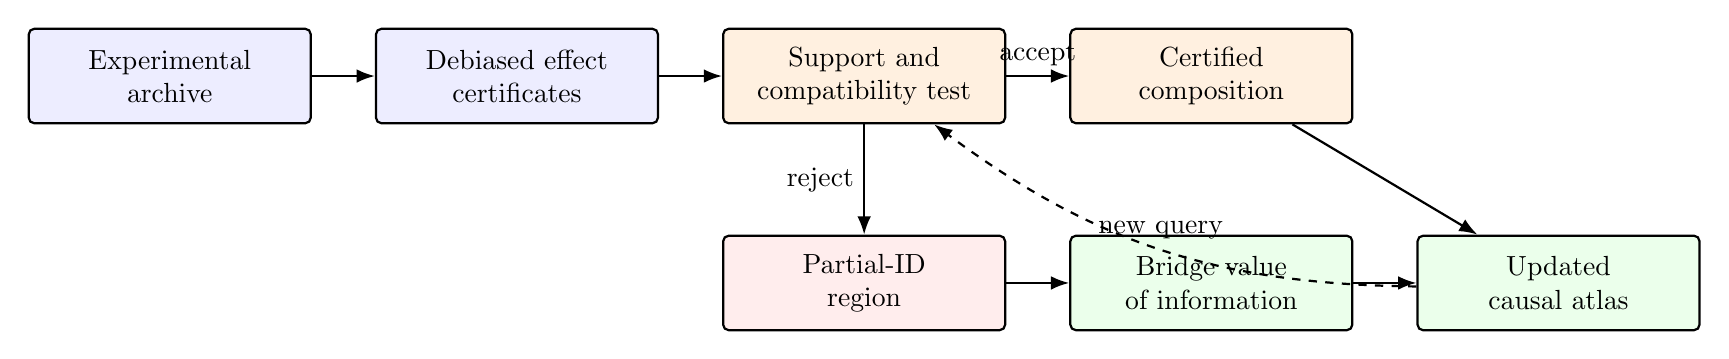
\begin{tikzpicture}[node distance=11mm and 8mm]
\node[bluebox] (archive) {Experimental\\archive};
\node[bluebox, right=of archive] (debias) {Debiased effect\\certificates};
\node[orangebox, right=of debias] (support) {Support and\\compatibility test};
\node[orangebox, right=of support] (transport) {Certified\\composition};
\node[redbox, below=14mm of support] (pid) {Partial-ID\\region};
\node[greenbox, right=of pid] (bridge) {Bridge value\\of information};
\node[greenbox, right=of bridge] (update) {Updated\\causal atlas};
\draw[arrow] (archive) -- (debias);
\draw[arrow] (debias) -- (support);
\draw[arrow] (support) -- node[above]{accept} (transport);
\draw[arrow] (transport) -- (update);
\draw[arrow] (support) -- node[left]{reject} (pid);
\draw[arrow] (pid) -- (bridge);
\draw[arrow] (bridge) -- (update);
\draw[dashedarrow] (update) to[bend left=18] node[above]{new query} (support);
\end{tikzpicture}}
\caption{A causal atlas is deliberately rejectable.  Semantic retrieval proposes candidate experiments; debiased uncertainty certificates, design compatibility, support, and moderator sensitivity decide whether composition is licensed.  Rejection produces a partial-identification region and a bridge-design objective rather than a forced point estimate.}
\label{fig:pipeline}
\end{figure}

\begin{algorithm}[H]
\caption{Rejectable Causal Atlas and Greedy Bridge Design}
\label{alg:atlas}
\begin{algorithmic}[1]
\Require Archive \(\cE_N\); target object \(e_\star\); candidate bridge library \(\cB\); budget \(B\); support tolerance \(\delta_{\rm sup}\); smoothness constants \(L,H\); confidence level \(1-\zeta\).
\Ensure Certified estimate, partial-identification interval, and/or selected bridge set.
\State Debias each archive effect using \eqref{eq:aipw-estimator}; store \((r_i,D_i,\cA_i,\widehat\tau_i,\cU_i)\).
\State Retrieve candidate set \(C\subseteq[N]\) by semantic and metadata screening.
\State Build the design signature for each candidate; apply every approved scale map to its estimate and uncertainty certificate.
\State Remove every \(j\in C\) with \(\kappa(e_j,e_\star)=0\), recording the failed field or missing map.
\If{\(C=\varnothing\)}
  \State \Return rejection with the broad target-effect bounds encoded by \(\cF_A\), and invoke bridge design.
\EndIf
\State Compute \(\widehat\alpha\) by the support program \eqref{eq:support-program}.
\State Compute the certificate radius \(Rad(\widehat\alpha,\zeta)\) from Theorem~\ref{thm:composition}.
\If{support residual, nuisance remainder, and moderator sensitivity imply \(Rad(\widehat\alpha,\zeta)\le \delta_{\rm sup}\)}
  \State \Return \(\widehat\theta_{\widehat\alpha}=\sum_{j\in C}\widehat\alpha_j\widehat\tau_j\) and the honest interval in Theorem~\ref{thm:asymptotic}.
\Else
  \State Construct \(\widehat\Theta_A(e_\star)\) from Theorem~\ref{thm:partial-id}.
  \State Initialize \(S_0=\varnothing\).
  \For{\(b=1,\ldots,B\)}
    \State Select \(u_b\in\argmax_{u\in\cB\setminus S_{b-1}}\widehat{\operatorname{VoI}}(u\mid S_{b-1})\).
    \State Set \(S_b=S_{b-1}\cup\{u_b\}\).
  \EndFor
  \State \Return partial-identification interval \(\widehat\Theta_A(e_\star)\) and bridge set \(S_B\).
\EndIf
\end{algorithmic}
\end{algorithm}

\section{Main Results}
\label{sec:theory}

The results are organized to mirror the operational logic of the causal atlas.  Section~\ref{sec:theory} first establishes the validity of the experiment-level evidence, then determines when those certified effects can be composed, and finally characterizes what the atlas should report when composition fails.

The first subsection, \emph{Debiased Archive Estimation}, records only the auxiliary variance envelope used by the composition analysis.  The standard AIPW unbiasedness and nuisance-remainder calculations are part of the method in Section~\ref{sec:method} and are derived in Appendix~\ref{app:aipw-calculation}, rather than being presented as a separate proposition.

The second subsection, \emph{Finite-Sample Composition}, establishes the central transport certificate.  Lemma~\ref{lem:wellposed} shows that the intersection of compatible certified intervals is a well-defined interval whenever the certificates are mutually consistent.  Theorem~\ref{thm:composition} then bounds the error of a transported composition by separating causal-support error, local curvature, hidden-moderator sensitivity, nuisance bias, and statistical noise.  The familiar fully observed affine identity is recorded only as a boundary case of this theorem rather than as a separate formal result.

The third subsection, \emph{Asymptotic Normality and Honest Confidence Intervals}, establishes the large-sample inferential behavior of an accepted composition.  Theorem~\ref{thm:asymptotic} gives both asymptotic normality and the resulting confidence interval, explicitly inflating the interval by the certified deterministic radius when approximation error is non-negligible.

The fourth subsection, \emph{Semantic Failure and Partial Identification}, establishes the boundary of semantic retrieval and the valid fallback after rejection.  Theorem~\ref{thm:impossibility} proves that observed-representation proximity alone cannot uniformly certify causal transport when relevant moderators are hidden.  The archive-induced partial-identification region and Theorem~\ref{thm:partial-id} then show that failed point composition can still produce a coverage-valid set of target effects rather than an unsupported point estimate.

The fifth subsection, \emph{Minimax Lower Bound}, establishes that this conservatism is information-theoretically necessary.  Theorem~\ref{thm:minimax} proves that unsupported targets incur an unavoidable geometric error, while finite archive noise contributes an additional information-limited term.  Thus, the error cannot be removed by replacing the atlas with a more sophisticated weighting algorithm alone.

The final subsection, \emph{Bridge Experiment Design}, turns the remaining unidentified region into an experimental-design objective.  The bridge value-of-information definition measures the expected reduction in the partial-identification diameter, and Theorem~\ref{thm:bridge} proves that greedy selection is near-optimal when this objective is monotone and weakly submodular, allowing for uniformly estimated marginal-value errors.

\subsection{Debiased Archive Estimation}

\begin{lemma}[Archive variance envelope]
\label{lem:variance-envelope}
Suppose Assumption~\ref{ass:identified} holds, the nuisance estimates are
cross-fitted with \(\widehat\pi_i\in[\pi_0,1-\pi_0]\),
\(\abs{Y_i}\le M\), and \(\widehat\mu_{i,a}\in[-M,M]\).  If the evaluation
scores are conditionally independent given a common external nuisance-training
sample, then for independent archive experiments and any \(\alpha\in\Delta_C\),
\[
  \Var\left(
    \sum_{j\in C}\alpha_j\widehat\tau_j
    \,\middle|\,
    \widehat\eta
  \right)
  \le
  \sum_{j\in C}\alpha_j^2\frac{C_M^2}{n_j},
  \qquad
  C_M=2M+\frac{2M}{\pi_0}.
\]
For ordinary fold-specific cross-fitting, the operational analogue is the
uncertainty certificate in Assumption~\ref{ass:noise}.
\end{lemma}

Thus the archive stores a debiased effect together with its nuisance and
variance certificates; the standard experiment-level facts serve the later
composition theorem without being presented as contributions of their own.

\subsection{Finite-Sample Composition}

For \(\alpha\in\Delta_C\), define the deterministic approximation radius
\begin{equation}
\label{eq:det-radius}
  D(\alpha)
  =
  L\rho_\star(\alpha)
  +\frac{H}{2}\sum_{j\in C}\alpha_j\norm{m_j-\bar m_\alpha}^2
  +R_{\rm hid}(\alpha)
  +\sum_{j\in C}\alpha_j\mathfrak b_j.
\end{equation}
The four terms are, respectively, causal support error, local curvature, hidden-moderator sensitivity, and nuisance-debiasing remainder.

\begin{lemma}[Well-posed atlas interval]
\label{lem:wellposed}
Let \(C\) be finite and let \(\cW_A(e_\star)\subseteq\Delta_C\) be a nonempty feasible weight set.  For any nonnegative radius function \(B:\cW_A(e_\star)\to[0,\infty)\), the set
\[
  \widehat\Theta_A(e_\star)
  =
  \bigcap_{\alpha\in\cW_A(e_\star)}
  \left[
  \sum_{j\in C}\alpha_j\widehat\tau_j-B(\alpha),
  \sum_{j\in C}\alpha_j\widehat\tau_j+B(\alpha)
  \right]
\]
is a closed interval whenever it is nonempty.  If it is empty, the archive estimates and the stated certificates are mutually inconsistent at the chosen confidence level.
\end{lemma}

\begin{theorem}[Finite-sample causal composition bound]
\label{thm:composition}
Let \(C\subseteq[N]\) satisfy \(\kappa(C,\star)=1\), and fix \(\alpha\in\Delta_C\).  Under Assumptions~\ref{ass:compatibility}--\ref{ass:moderator}, with probability at least \(1-\zeta\),
\begin{equation}
\label{eq:composition-bound}
\begin{aligned}
\abs{\tau_\star-\sum_{j\in C}\alpha_j\widehat\tau_j}
&\le
L\rho_\star(\alpha)
+\frac{H}{2}\sum_{j\in C}\alpha_j\norm{m_j-\bar m_\alpha}^2
+R_{\rm hid}(\alpha)
+\sum_{j\in C}\alpha_j\mathfrak b_j \\
&\quad
+\sqrt{2\log(2/\zeta)\sum_{j\in C}\alpha_j^2s_j^2}
\equiv Rad(\alpha).
\end{aligned}
\end{equation}
If the archive experiments have a certified sub-Gaussian proxy matrix \(\Sigma\) instead of conditional independence, the statistical term is replaced by \(\sqrt{2\log(2/\zeta)\alpha^\top\Sigma\alpha}\).
\end{theorem}

\noindent\textbf{Scientific reading.}
The theorem says that reuse is valid only when five quantities are controlled.  The target must lie in causal support, the effect surface must be nearly linear over the local hull, the archived estimates must be precise, the debiasing remainder must be small, and omitted moderators must be certified.  It does not say that semantic neighbors are valid; semantic retrieval merely supplies candidates.

\paragraph{Affine boundary case.}
The familiar semantic-atlas identity follows directly from
Theorem~\ref{thm:composition}, so we do not elevate it to a separate result.
If \(r(e)=m(e)\), \(R_{\rm hid}(\alpha)=0\), \(\mathfrak b_j=0\),
\(\kappa(C,\star)=1\), \(\mu\) is affine on the relevant convex hull, and
\(m_\star=\sum_{j\in C}\alpha_jm_j\), then
\[
  \tau_\star=\sum_{j\in C}\alpha_j\tau_j.
\]
With estimated archive effects, the only remaining term in
\eqref{eq:composition-bound} is statistical.  This boundary case clarifies
why semantic composition can work under causal sufficiency without presenting
the classical affine identity as a standalone contribution.

\subsection{Asymptotic Normality and Honest Confidence Intervals}

Let \(\theta_\alpha=\sum_{j\in C}\alpha_j\tau_j\) and \(V_{\alpha,n}=\sum_{j\in C}\alpha_j^2v_j/n_j\).  The next theorem separates statistical normality around the composed archive estimand \(\theta_\alpha\) from approximation bias relative to \(\tau_\star\).

\begin{theorem}[Asymptotic distribution and honest interval for an accepted composition]
\label{thm:asymptotic}
Consider a triangular sequence of archives with candidate sets \(C_n\) and
weights \(\alpha_n\). Suppose Assumptions~\ref{ass:identified}--
\ref{ass:moderator} hold. Write
\[
  \psi_{j\ell}
  =
  \phi_j(W_{j\ell};\eta_j)-\tau_j,
  \qquad
  v_j=\Var(\psi_{j\ell}),
\]
and suppose the cross-fitted estimators admit the aggregate asymptotic
linear expansion
\[
  \widehat\tau_j-\tau_j
  =
  \frac{1}{n_j}\sum_{\ell=1}^{n_j}\psi_{j\ell}
  +
  r_{j,n},
  \qquad
  \sum_{j\in C_n}\alpha_{n,j}r_{j,n}
  =
  o_{\Pbb}(V_{\alpha,n}^{1/2}),
\]
where
\[
  V_{\alpha,n}
  =
  \sum_{j\in C_n}\alpha_{n,j}^2\frac{v_j}{n_j}.
\]
This remainder condition is the precise aggregate nuisance-rate
requirement used in the proof; it is typically obtained from cross-fitting
and the product-rate calculation in Appendix~\ref{app:aipw-calculation}. Assume the
independent influence-function summands satisfy the Lindeberg condition
\[
  \frac{1}{V_{\alpha,n}}
  \sum_{j\in C_n}\frac{\alpha_{n,j}^2}{n_j}
  \E\left[
    \{\phi_j(W_j;\eta_j)-\tau_j\}^2
    \1\left\{
      \abs{\alpha_{n,j}
      (\phi_j(W_j;\eta_j)-\tau_j)/n_j}
      >
      \eps V_{\alpha,n}^{1/2}
    \right\}
  \right]
  \to0
\]
for every \(\eps>0\). Then
\begin{equation}
\label{eq:clt-theta}
  \frac{\widehat\theta_{\alpha_n}-\theta_{\alpha_n}}
       {V_{\alpha,n}^{1/2}}
  \rightsquigarrow
  \Normal(0,1).
\end{equation}
If \(\widehat V_{\alpha,n}/V_{\alpha,n}\to_{\Pbb}1\), the studentized
statistic is also asymptotically standard normal. Moreover, if the
deterministic approximation radius
\(D(\alpha_n)=o(V_{\alpha,n}^{1/2})\), then
\[
  \frac{\widehat\theta_{\alpha_n}-\tau_\star}
       {V_{\alpha,n}^{1/2}}
  \rightsquigarrow
  \Normal(0,1).
\]
Suppressing the sequence index in the following display, and without requiring
\(D(\alpha_n)=o(V_{\alpha,n}^{1/2})\), define
\begin{equation}
\label{eq:honest-ci}
  \operatorname{CI}_{1-\zeta}(\alpha)
  =
  \left[
    \widehat\theta_\alpha
    -z_{1-\zeta/2}\widehat V_\alpha^{1/2}
    -\widehat D(\alpha),
    \widehat\theta_\alpha
    +z_{1-\zeta/2}\widehat V_\alpha^{1/2}
    +\widehat D(\alpha)
  \right]
\end{equation}
This interval has asymptotic coverage at least \(1-\zeta\) whenever the one-sided radius
underestimation is negligible:
\[
  \frac{\{D(\alpha)-\widehat D(\alpha)\}_+}
       {V_\alpha^{1/2}}
  \xrightarrow{\Pbb}
  0.
\]
This condition permits conservative overestimation of \(D(\alpha)\) and
rules out only first-order underestimation. If
\(D(\alpha)=o(V_\alpha^{1/2})\), the shorter Wald interval without
\(\widehat D(\alpha)\) is valid.
\end{theorem}

This is the inferential boundary of the atlas.  A target in sufficiently good causal support receives an ordinary asymptotic confidence interval.  A target with nonnegligible support or moderator error receives an honest interval inflated by \(\widehat D(\alpha)\).  A target whose inflated interval is too wide is routed to partial identification and bridge design.

\subsection{Semantic Failure and Partial Identification}

\begin{theorem}[Semantic proximity is insufficient under hidden moderators]
\label{thm:impossibility}
Let \(x(e)\) be an observed representation for which there exist two admissible experiments \(e^0,e^1\) with \(x(e^0)=x(e^1)\) but \(h(e^0)\ne h(e^1)\) for a moderator coordinate \(h\) allowed by the model class.  Then for every \(\eta>0\), there exists an effect surface \(\mu\) satisfying Assumption~\ref{ass:smooth} and two targets with \(\norm{x(e^0)-x(e^1)}\le\eta\) but
\[
  \abs{\tau(e^1)-\tau(e^0)}\ge c
\]
for a constant \(c>0\) determined by the moderator range and the Lipschitz radius.  Hence no procedure based only on \(x\)-distance can uniformly certify causal composability over this model class.
\end{theorem}

A common objection is that a sufficiently strong embedding could include the moderator.  That objection is correct and is precisely why the theorem is useful.  If the representation is causally sufficient, the theorem does not apply and the affine boundary case following Theorem~\ref{thm:composition} describes the favorable setting.  The impossibility concerns representations that are many-to-one over moderators relevant to treatment effects.

\begin{definition}[Archive-induced partial-identification region]
Let \(\cF_A\) be the class of effect surfaces satisfying the stated smoothness, design-compatibility, moderator, and uncertainty certificates.  The archive-induced partial-identification region for the target is
\[
  \Theta_A(e_\star)=\{f(m_\star):f\in\cF_A\}.
\]
\end{definition}

\begin{theorem}[Valid partial identification from failed composition]
\label{thm:partial-id}
Assume the conditions of Theorem~\ref{thm:composition}.  Let \(\cW_A(e_\star)\) be a finite collection of design-compatible weights and choose confidence levels \(\{\zeta_\alpha:\alpha\in\cW_A(e_\star)\}\) with \(\sum_{\alpha\in\cW_A(e_\star)}\zeta_\alpha\le\zeta\).  Define
\begin{equation}
\label{eq:pid-est}
  \widehat\Theta_A(e_\star)
  =
  \bigcap_{\alpha\in\cW_A(e_\star)}
  \left[
  \sum_j\alpha_j\widehat\tau_j-Rad(\alpha,\zeta_\alpha),
  \sum_j\alpha_j\widehat\tau_j+Rad(\alpha,\zeta_\alpha)
  \right],
\end{equation}
where \(Rad(\alpha,u)\) denotes the right-hand side of \eqref{eq:composition-bound} with confidence argument \(u\).  Then
\[
  \Pbb\{\tau_\star\in\widehat\Theta_A(e_\star)\}\ge1-\zeta.
\]
Moreover, if every design-compatible convex combination has support residual at least \(r_0>0\), then point identification is impossible over the Lipschitz class without an additional restriction: there exist two admissible effect surfaces agreeing on the archive and differing at \(m_\star\) by at least \(c_0\min\{Lr_0,M\}\), where \(M\) is the global effect bound and \(c_0>0\) is universal.
\end{theorem}

Failed composition is therefore not a failed method.  It is a certificate that the archive does not contain the target mechanism at the requested resolution.  The width of \(\widehat\Theta_A(e_\star)\) quantifies the missing bridge.

\subsection{Minimax Lower Bound}

The previous theorem states non-identification.  The next result states an information-theoretic lower bound.  It shows that the atlas certificate is not merely conservative: its support and variance terms are unavoidable in the worst case.

\begin{theorem}[Minimax lower bound for unsupported targets]
\label{thm:minimax}
Fix a design-compatible archive hull \(K=\conv\{m_j:j\in C,\kappa(e_j,e_\star)=1\}\) and let \(d_\star=\dist(m_\star,K)\).  Consider the Gaussian archive experiment
\[
  Z_j=\mu(m_j)+\varepsilon_j,
  \qquad
  \varepsilon_j\ind \Normal(0,s_j^2),
  \qquad j\in C,
\]
with known \(s_j^2\).  Let \(\cF(L,M)\) be the class of functions \(\mu:\cM\to[-M,M]\) that are \(L\)-Lipschitz.  Then for a universal constant \(c>0\),
\begin{equation}
\label{eq:minimax-bound}
  \inf_{\widehat T}
  \sup_{\mu\in\cF(L,M)}
  \E_\mu\abs{\widehat T-\mu(m_\star)}
  \ge
  c\left[
    \{Ld_\star\}\wedge M
    \ \vee\
    \left\{\sum_{j\in C}s_j^{-2}\right\}^{-1/2}\wedge M
  \right].
\end{equation}
If \(d_\star>0\), no estimator can uniformly remove the geometric support error without adding assumptions beyond \(\cF(L,M)\).  If \(d_\star=0\), the remaining lower bound is the usual Fisher-information term for estimating a common local level.
\end{theorem}

The lower bound explains why the atlas reports partial identification instead of extrapolating.  When the target lies outside the design-compatible hull, the error floor is geometric, not computational.  Better algorithms cannot recover an unsupported effect; only stronger assumptions or a bridge experiment can.

\subsection{Greedy Bridge-Design Guarantee}

The Method section defines the bridge value of information and the adaptive greedy rule.  This subsection establishes when that rule is close to the best policy available in the finite bridge library.

\begin{theorem}[Greedy adaptive bridge-design guarantee]
\label{thm:bridge}
Let \(\cB\) be a finite bridge library.  For \(S\subseteq\cB\), write
\[
  F(S)=\diam\{\Theta_A(e_\star)\}-\E[\diam\{\Theta_{A\cup S}(e_\star)\}].
\]
Assume \(F\) is monotone, \(F(\varnothing)=0\), and \(\gamma\)-weakly submodular:
\[
  \sum_{b\in T\setminus S}\{F(S\cup\{b\})-F(S)\}
  \ge
  \gamma\{F(T)-F(S)\}
\]
for all \(S\subseteq T\subseteq\cB\).  Suppose greedy bridge design selects elements using estimated marginal values whose uniform absolute error is at most \(\eps_{\rm est}\).  If \(S_B\) is the greedy set after \(B\) bridges and \(S^\star\in\argmax_{|S|\le B}F(S)\), then
\begin{equation}
\label{eq:bridge-bound}
  F(S_B)
  \ge
  (1-e^{-\gamma})F(S^\star)-\frac{2B\eps_{\rm est}}{\gamma}.
\end{equation}
Equivalently,
\[
  \E[\diam\{\Theta_{A\cup S_B}(e_\star)\}]
  \le
  \diam\{\Theta_A(e_\star)\}
  -(1-e^{-\gamma})F(S^\star)
  +\frac{2B\eps_{\rm est}}{\gamma}.
\]
\end{theorem}

The theorem does not assert that every scientific bridge objective is submodular.  It says that when bridge effects have approximate diminishing returns, a greedy atlas policy is near-optimal for shrinking the unidentified region.  This is why the empirical section evaluates bridge selection by partial-identification diameter rather than by semantic novelty.

\section{Experiments: Synthetic and Real-World Analysis}
\label{sec:experiments}

The experiments are designed to test the theory rather than to decorate it.  Each reported table corresponds to a theoretical object.  Reconstruction error tests the composition bound; coverage tests uncertainty calibration; rejection rate tests support diagnostics; interval width tests partial identification; bridge shrinkage tests Theorem~\ref{thm:bridge}; sensitivity curves stress Assumption~\ref{ass:moderator}.

\subsection{Experimental Setup}
\paragraph{Synthetic data-generating process.}
Each synthetic archive contains eight randomized experiments.  The mechanism is $m=(s_1,s_2,h,q)\in[-1,1]^4$, where $s_1$ and $s_2$ are public semantic coordinates, $h$ is a hidden moderator observed through a bounded proxy, and $q$ records a design/context coordinate.  A nonlinear effect surface with interactions and curvature generates the experiment-level effects.  Every nominal experiment contains 400 units with treatment probability $0.5$; the target also contains 400 units and is used only to supply the synthetic truth after prediction.  This construction permits semantic neighbors to be causally incompatible through variation in $h$ and $q$.  The complete surface, proxy construction, analytic bounds, and optimizer constants are given in 
Appendix~\ref{app:synthetic-dgp}.
\paragraph{Methods and baselines.}
The proposed Causal ATLAS uses the full public causal representation, design compatibility, estimated effect uncertainty, and the declared moderator certificate.  We compare it with the same composition forced to release every target, semantic forced composition using only $(s_1,s_2)$, nearest semantic retrieval, and a global archive mean.  The shared-target benchmark additionally includes an evaluation-only oracle latent-support reference: it replaces the public representation by the simulated latent mechanism, but it is unavailable to any deployable procedure and is never used for retrieval, weighting, release, or bridge selection.  Complete formal ablations for removing the variance penalty and restricting retrieval to four candidates are reported in Appendix~\ref{app:formal-ablations}.

\paragraph{Metrics and protocol.}
We pool three prespecified seed batches and 100 target draws per seed.  All methods receive the same archive--target draw whenever they are compared.  We report release rate, MAE, RMSE, and sign accuracy, with point-error metrics for a rejectable method conditioned on release.  Interval coverage is always reported jointly with mean width.  For a released subset $\mathcal R$, the selective risk is
\[
\operatorname{MAE}_{\mathrm{released}}
 =\mathbb E\!\left[\abs{\widehat\tau-\tau^\star}\mid \text{release}\right],
\]
which is not an unconditional accuracy claim.  Partial-identification diameter is evaluated on rejected targets, and bridge quality is the reduction in that same diameter.  The repository retains seed-wise summaries and Monte Carlo errors; the main section emphasizes effect sizes and the behavior of the decision rule.


\subsection{Certified Causal Composition}
The shared-target benchmark shows that causal composition and abstention work together.  Causal ATLAS releases $0.463$ of the 300 common targets and has released-target MAE $0.111$, whereas forcing the same weights to publish all targets gives MAE $0.139$ (Table~\ref{tab:v1-main-synthetic}).  The oracle latent-support reference has MAE $0.135$ on the full target population.  The released ATLAS subset and the full-population oracle are therefore not directly comparable as unconditional risks; the fair representation comparison is between ATLAS with and without rejection.  Semantic forced, nearest semantic, and global mean have MAEs $0.249$, $0.553$, and $0.282$, respectively.
\begin{figure}[t]
\centering
\includegraphics[width=\textwidth]{experiments/causal_atlas_bridge/figures/figure2_composability.pdf}
\caption{Why causal composability requires more than semantic similarity.  \textbf{(a)} Semantic neighbors can differ in the hidden moderator.  \textbf{(b)} Full absolute-error distributions for the six shared-target methods; the released ATLAS curve is conditional on the 139 released targets.  \textbf{(c)} Representation advantage $\Delta_{\rm rep}=\mathrm{MAE}_{\rm semantic}-\mathrm{MAE}_{\rm ATLAS,no\text{-}rejection}$ over hidden shift and proxy uncertainty.  \textbf{(d)} Certificate radius versus realized ATLAS error; the release threshold is shown for diagnosis.  Bridge design is intentionally absent here and appears in Figure 4.}
\label{fig:v1-composition}
\end{figure}
\begin{table}[H]
\centering
\caption{Shared-target synthetic benchmark on the same 300 target draws. The evaluation population is explicit: Causal ATLAS point metrics are conditional on its released targets (139 of 300), whereas ATLAS without rejection, all forced baselines, and the evaluation-only latent oracle are evaluated on all 300 targets. The released ATLAS MAE is therefore not directly comparable with the all-target oracle MAE.}
\label{tab:v1-main-synthetic}
\resizebox{\textwidth}{!}{%
\begin{tabular}{llrrrrrr}
\toprule
Method & Evaluation population & Release & MAE & RMSE & Sign & Coverage & Width \\
\midrule
Causal ATLAS & Released targets (139/300) & 0.463 & 0.111 & 0.138 & 0.928 & 1.000 & 2.946 \\
ATLAS, no rejection & All targets (300/300) & 1.000 & 0.139 & 0.170 & 0.893 & 1.000 & 3.339 \\
Semantic forced & All targets (300/300) & 1.000 & 0.249 & 0.310 & 0.797 & 1.000 & 2.831 \\
Nearest semantic & All targets (300/300) & 1.000 & 0.553 & 0.697 & 0.717 & 0.970 & 3.127 \\
Global mean & All targets (300/300) & 1.000 & 0.282 & 0.362 & 0.780 & 1.000 & 3.564 \\
Oracle latent support$^{\dagger}$ & All targets (300/300) & 1.000 & 0.135 & 0.160 & 0.893 & 1.000 & 3.337 \\
\bottomrule
\end{tabular}
}
\begin{minipage}{0.96\linewidth}\footnotesize
$^{\dagger}$ The oracle replaces the public representation with simulated latent mechanisms and is evaluation-only; it is unavailable to retrieval, weighting, release, or bridge selection.
\end{minipage}
\end{table}

Figure~\ref{fig:v1-composition} explains why the mean comparison is not merely a semantic-neighbor result.  Targets can be close in $(s_1,s_2)$ while differing materially in $h$, so methods that use only semantic coordinates exhibit heavier error tails than the design-enriched representation.  The behavior is consistent with the non-identifiability phenomenon in Theorem~\ref{thm:impossibility}; it is an empirical illustration rather than a proof of that theorem.

The representation sensitivity grid isolates this mechanism by disabling rejection in the ATLAS-versus-semantic comparison.  At proxy uncertainty $0.10$, increasing the hidden shift from $0$ to $0.8$ increases $\Delta_{\rm rep}$ from $0.123$ to $0.603$.  At the same time, the ATLAS release rate falls from $0.887$ to $0.260$.  Thus a representation can improve prediction while the certificate correctly determines that fewer targets have enough support for release.

Finally, the certificate radius has Spearman correlation $0.272$ with realized absolute error across the 300 common targets.  The association is positive but moderate: the certificate is informative about target difficulty without being a pointwise error predictor.  No realized error exceeds the reported certificate radius in this diagnostic set.  We treat this as an empirical diagnostic, not as a theorem-violation test, because the plotted finite-sample event is not asserted to be identical to the probability event in the guarantee.
\subsection{Selective Prediction and Honest Uncertainty}
Selective prediction must be evaluated as a risk--coverage tradeoff rather than as a single conditional error.  Holding the same 300 nominal targets fixed and changing only the scientific tolerance gives release rates $0.010$, $0.500$, and $0.943$ at thresholds $1.25$, $1.65$, and $2.00$, with conditional MAEs $0.074$, $0.116$, and $0.133$; the no-rejection endpoint has MAE $0.136$ (Figure~\ref{fig:v1-calibration}a).  Relaxing the threshold therefore exposes an explicit frontier instead of hiding the cost of abstention.
\begin{figure}[t]
\centering
\includegraphics[width=\textwidth]{experiments/causal_atlas_bridge/figures/figure3_uncertainty.pdf}
\caption{Selective prediction and honest uncertainty.  \textbf{(a)} Risk--coverage frontier on a fixed target set.  \textbf{(b)} Nominal versus empirical coverage for honest ATLAS and Wald-only intervals.  \textbf{(c)} Mean interval width accompanying the same confidence levels.  \textbf{(d)} Released-target (conditional) interval coverage under strong and severe mismatch when smoothness is deliberately understated. Certified ATLAS coverage is conditional on release; forced policies release all targets, so their released-target coverage is also their all-target coverage. The honest interval is conservative because it retains approximation and moderator uncertainty; Wald-only omits those components.}
\label{fig:v1-calibration}
\end{figure}
Across nominal confidence levels $0.80$, $0.90$, $0.95$, and $0.975$, the honest intervals have empirical coverage $1.000$ while mean width increases from $3.283$ to $3.367$.  The relevant comparison is not coverage alone: Wald-only intervals have coverage only $0.200$, $0.240$, $0.287$, and $0.337$, with widths below $0.20$.  Sampling uncertainty alone is therefore insufficient for archive transport.

The negative-control experiments make the assumption boundary explicit.  Under strong and severe semantic mismatch, deliberately understating the smoothness bounds lowers coverage to $0.833$ and $0.723$, respectively, while the certified procedure continues to reject almost all unsupported targets and retains conservative coverage on the released branch.  The conclusion is conditional: the guarantees depend on valid certificate components, and a numerically narrow but misspecified certificate can be overconfident.
\subsection{From Rejection to Partial Identification}
Rejection is not a terminal failure.  We move the target toward a fixed in-domain anchor and, after a point prediction is rejected, return the Theorem~\ref{thm:partial-id} partial-identification interval.  As support deteriorates, the rejection rate increases from $0.517$ to $0.990$, while the average PI diameter on rejected targets increases from $3.646$ to $7.076$ (Table~\ref{tab:v1-partial-id}).
All rejected-branch intervals contain the simulated truth in the prespecified scenarios, and all intersections are nonempty.  The width increase is therefore the intended expression of loss of identification rather than a numerical failure.  In short,
\[
\text{support worsens}
\;\Rightarrow\;
\text{release decreases}
\;\Rightarrow\;
\text{the identified set widens}.
\]
\begin{table}[H]
\centering
\caption{Support deterioration, rejection, and partial identification (PI) under the shared-target support-stress protocol. All PI quantities are evaluated on rejected synthetic targets.}
\label{tab:v1-partial-id}
\begin{tabular}{lrrrr}
\toprule
Scenario & Rejection & Nonempty PI & PI coverage & PI diameter \\
\midrule
Nominal support & 0.517 & 1.000 & 1.000 & 3.646 \\
Moderate mismatch & 0.777 & 1.000 & 1.000 & 4.095 \\
Strong mismatch & 0.973 & 1.000 & 1.000 & 5.674 \\
Severe mismatch & 0.990 & 1.000 & 1.000 & 7.076 \\
\bottomrule
\end{tabular}
\end{table}

\begin{figure}[t]
\centering

\includegraphics[width=\textwidth]{experiments/causal_atlas_bridge/figures/figure4_rejection_bridge.pdf}
\caption{From failed composition to experiment design.  \textbf{(a)} Release probability as the target-shift/support-stress parameter $\rho$ changes; $\rho$ is evaluation-only.  \textbf{(b)} PI diameter among rejected targets as the same evaluation-only $\rho$ changes.  \textbf{(c)} Sequential bridge-budget paths in the severe-mismatch diagnostic; the lines use a focused 90-path visualization, while the formal claims use 300 repetitions.  Black diamonds are ex-post exhaustive values and are evaluation-only.}
\label{fig:v1-support-bridge}
\end{figure}
\subsection{Bridge Experiment Design}
Once composition is rejected, the next question is not how to extrapolate harder, but which experiment should be run next.  The bridge planner evaluates the conditional marginal expected reduction in the current PI diameter, selects a candidate, observes its noisy effect, and recomputes the remaining values.  We compare causal-support greedy selection with semantic-only greedy and uniform random selection under a budget of four.

In the severe-mismatch formal experiment, causal greedy reduces the mean diameter from $6.942$ to $1.877$, a $72.96\%$ reduction.  Semantic greedy and random finish at $2.331$ and $2.317$, respectively, so their performance is substantially closer to each other than to the causal-support policy.  The focused path in Figure~\ref{fig:v1-support-bridge}c shows the same ordering while exposing the budget trajectory.

For the small candidate library where ex-post enumeration is feasible, greedy attains $0.9957$, $0.9776$, and $0.9857$ of the exhaustive bridge value at budgets $1$, $2$, and $3$.  Because the exhaustive comparator uses realized bridge outcomes, it is not deployable and does not estimate a weak-submodularity parameter or prove the coefficient in Theorem~\ref{thm:bridge}.
\subsection{Real-Data NSW Archive}

The real-data evaluation uses the Dehejia--Wahba NSW job-training data \citep{lalonde1986evaluating,dehejia1999causal}.  We use the randomized NSW job-training data as a reconstruction stress test rather than as a setting with known subgroup-level causal ground truth.  Local archive objects are constructed from covariate neighborhoods with minimum treated and control support; held-out objects are reconstructed from the remaining archive.  The held-out local contrast is a noisy reference quantity, not the true conditional treatment effect.

% Paper-facing layout; numeric values are from committed NSW result records.
\begin{table}[t]
\centering
\small
\setlength{\tabcolsep}{3.5pt}
\caption{NSW held-out local-contrast reconstruction. All-target MAE uses all 1,680 raw reconstructions; Released MAE uses released targets only. Inclusion refers to a noisy held-out local contrast, not a latent subgroup effect; monetary quantities are thousands of U.S. dollars.}
\label{tab:v1-nsw}
\begin{tabular}{lrrrrrrr}
\toprule
Method & All-target MAE & Released MAE & Median AE & Sign & Inclusion & Width & Rejection \\
\midrule
Causal ATLAS & 0.862 & 0.864 & 0.699 & 0.854 & 0.974 & 5.630 & 0.232 \\
ATLAS, no rejection & 0.862 & 0.862 & 0.699 & 0.854 & 0.970 & 5.275 & 0.000 \\
Semantic forced & 1.169 & 1.169 & 0.937 & 0.754 & 0.605 & 2.854 & 0.000 \\
Nearest semantic & 1.242 & 1.242 & 1.031 & 0.780 & 0.992 & 8.311 & 0.000 \\
Global mean & 1.679 & 1.679 & 1.349 & 0.784 & 0.446 & 2.475 & 0.000 \\
\bottomrule
\end{tabular}
\end{table}


\begin{figure}[t]
\centering

\includegraphics[width=\textwidth]{experiments/causal_atlas_bridge/figures/figure5_nsw.pdf}
\caption{NSW reconstruction and certificate diagnostics.  \textbf{(a)} PCA map of the 112 local archive objects, colored by ATLAS release frequency.  \textbf{(b)} Held-out reconstruction against noisy local contrasts, with accepted and rejected targets separated.  \textbf{(c)} Certificate radius versus reconstruction error, colored by reported interval width.  Inclusion is reference inclusion, not coverage of a latent subgroup effect.}
\label{fig:v1-nsw}
\end{figure}

Causal ATLAS obtains MAE $0.862$, median absolute error $0.699$, sign accuracy $0.854$, held-out reference inclusion $0.974$, width $5.630$, and rejection rate $0.232$.  Semantic forced and global mean are narrower but include the held-out reference only $0.605$ and $0.446$ of the time, whereas nearest semantic reaches $0.992$ inclusion with width $8.311$.  Point-error metrics are computed on all raw reconstructions, so Causal ATLAS and its no-rejection counterpart have identical point metrics; they differ only in release and certification.  These results reproduce the reconstruction--certification tradeoff in a heterogeneous archive, not a real-world causal generalization claim.

The archive map and target-level diagnostics show that reconstruction becomes harder in sparsely supported regions.  Local objects overlap, so their estimated effects are statistically dependent; the current experiment is descriptive and does not implement a full shared-unit covariance correction.  The results therefore support the practical behavior of the framework while leaving external validity, alternative neighborhood definitions, and nuisance-estimation uncertainty for future work.

Across the synthetic experiments, Causal ATLAS improves composition when causal support is informative, exposes a transparent risk--coverage frontier, and protects interval validity when its declared uncertainty bounds are correct.  When support is insufficient, it transitions to partial identification instead of forced extrapolation; bridge experiments then shrink the resulting diameter.  NSW is consistent with these mechanisms as a reconstruction stress test, while supplying no causal ground truth for subgroup effects.



\section{Discussion}
\label{sec:discussion}

This paper draws a boundary around what an experimental archive can and cannot do.  If the representation is causally sufficient, the design profiles are compatible, and the target lies in local support, then the archive can produce a debiased, certified transported effect.  If a relevant moderator is omitted, semantic proximity is not enough.  The correct output is a partial-identification region, a sensitivity statement, and a bridge-design recommendation.

The limitations are best understood as new research questions.  First, the mechanism representation is treated as supplied by diagnostics, metadata, and analyst encoding.  Learning such representations from multimodal experiment descriptions requires separate identifiability conditions; this is not a mere representation-learning problem because omitted moderators induce non-identification.  Second, local smoothness is a scope condition rather than a universal law.  Negative controls, placebo outcomes, moderator curves, and sensitivity analysis should be used to decide where smoothness is credible.  Third, bridge value is computed over a finite candidate library.  Designing the library itself is an experimental-design problem: one must choose which populations, treatment intensities, outcomes, and control conditions could most efficiently close the support gap.

The broader implication is that scientific discovery engines should be allowed to say no.  A system that always returns a point estimate hides the distinction between evidence reuse and extrapolation.  A causal atlas makes that distinction explicit.  It can say: this effect transports; this effect is only partially identified; and this is the bridge experiment that would change the answer.  In the Causal ATLAS roadmap, this paper supplies the first module: archive-to-discovery evidence reuse with honest refusal.  Later modules can build on it for LLM-generated treatments, regret-calibrated assignment, causal routing, dynamic networks, strategic AI systems, geometric identifiability, and discovery engines.

\appendix

\section{Appendix: Notation and Proofs}
\label{app:proofs}

\subsection{Notation Table}

\begin{table}[H]
\centering
\small
\caption{Core notation used in the proofs.}
\begin{tabular}{ll}
\toprule
Symbol & Meaning \\
\midrule
\(e_i\) & Archived experiment object \\
\(e_\star\) & Target experiment object \\
\(W_{i\ell}\) & Unit record \((X_{i\ell},A_{i\ell},Y_{i\ell})\) in experiment \(i\) \\
\(n_i\) & Sample size of experiment \(i\) \\
\(m_i,m_\star\) & Latent causal mechanism vectors in \(\cM\subset\R^p\) \\
\(r_i,r_\star\) & Observed atlas representations \\
\(\tau_i,\tau_\star\) & True causal effects \(\mu(m_i),\mu(m_\star)\) \\
\(\widehat\tau_i\) & Debiased archive effect estimate \\
\(\cU_i=(n_i,\widehat v_i,\mathfrak b_i)\) & Experiment-level uncertainty certificate \\
\(\mu\) & Effect surface on the mechanism space \\
\(\kappa(C,\star)\) & Design-compatibility predicate for candidate set \(C\) and target \\
\(\Delta_C\) & Simplex over candidate experiments \(C\) \\
\(\alpha\) & Composition weights \\
\(\bar m_\alpha\) & Weighted mechanism \(\sum_{j\in C}\alpha_jm_j\) \\
\(\rho_\star(\alpha)\) & Causal support residual \(\norm{m_\star-\bar m_\alpha}\) \\
\(R_{\rm hid}(\alpha)\) & Hidden-moderator sensitivity residual \\
\(\mathfrak b_i\) & Second-order nuisance-bias bound for experiment \(i\) \\
\(\Theta_A(e_\star)\) & Archive-induced partial-identification region \\
\(\operatorname{VoI}_A(b)\) & Bridge value of information for candidate bridge \(b\) \\
\bottomrule
\end{tabular}
\end{table}



The appendix follows the logical order of the main results.  It first gives
the standard conditional-unbiasedness and nuisance-error calculation used to
construct \(\mathfrak b_i\), followed by the proof of the auxiliary variance
envelope in Lemma~\ref{lem:variance-envelope}.  It then verifies the interval
construction in Lemma~\ref{lem:wellposed} and proves the finite-sample
composition certificate in Theorem~\ref{thm:composition}.  The classical
affine boundary case needs no separate proof.  The normalized triangular-array
and confidence-interval arguments are presented together as the proof of
Theorem~\ref{thm:asymptotic}.  The remaining subsections prove the semantic
boundary, partial-identification, minimax, and bridge-design results in their
order of appearance.

\subsection{AIPW Orthogonality and Nuisance-Remainder Calculation}
\label{app:aipw-calculation}

\paragraph{Proof strategy.} We condition on the nuisance-training folds first.  The proof then evaluates one score at a time, derives its conditional mean, and controls the second-order remainder used in the composition radius.

The score used throughout this proof is the AIPW score in
\eqref{eq:aipw-score}, while its cross-fitted average is the estimator in
\eqref{eq:aipw-estimator}.  We first establish the conditional-unbiasedness
claim in \eqref{eq:app-proof-002}, then derive the nuisance product remainder
in \eqref{eq:app-proof-010}.

Fix an experiment \(i\) and suppress the subscript.  Let \(I_1,\ldots,I_K\) be its evaluation folds, let \(\mathcal T_k\) be the data used to train the nuisance functions applied on \(I_k\), and write \(\widehat\tau_k\) for the fold average.  Cross-fitting ensures that, conditional on \(\mathcal T_k\), the fitted functions are fixed and the observations in \(I_k\) retain their evaluation law.  Write \(\mu_a(x)=\E(Y\mid A=a,X=x)=\E\{Y(a)\mid X=x\}\), where the last equality follows from consistency and ignorability.  Conditional on the cross-fitting training folds, the nuisance functions entering the score are fixed functions of \(x\).  For arbitrary fixed functions \(\widehat\mu_0,\widehat\mu_1\) and the true propensity \(\pi\), define
\begin{equation}
\label{eq:app-proof-001}
\phi(W;\widehat\mu_0,\widehat\mu_1,\pi)
  =
  \widehat\mu_1(X)-\widehat\mu_0(X)
  +\frac{A\{Y-\widehat\mu_1(X)\}}{\pi(X)}
  -\frac{(1-A)\{Y-\widehat\mu_0(X)\}}{1-\pi(X)}.
\end{equation}
The display in \eqref{eq:app-proof-001} defines the single-observation score.
For known propensities, the precise claim needed for ordinary cross-fitting is the foldwise conditional identity 
\begin{equation}
\label{eq:app-proof-002}
\E\{\widehat\tau_k\mid\mathcal T_k\}=\tau,
\qquad
\widehat\tau_k
=\frac{1}{|I_k|}\sum_{\ell\in I_k}
\phi(W_\ell;\widehat\mu_0^{(-k)},\widehat\mu_1^{(-k)},\pi).
\end{equation}
Conditioning on \(\mathcal T_k\) permits the fold-average reduction in \eqref{eq:app-proof-003}.  We then condition once more on \(X\) to evaluate a generic score,
\begin{equation}
\label{eq:app-proof-003}
\begin{aligned}
\E(\widehat\tau_k\mid\mathcal T_k)
&=\frac{1}{|I_k|}\sum_{\ell\in I_k}
  \E\!\left\{
  \phi(W_\ell;\widehat\mu_0^{(-k)},\widehat\mu_1^{(-k)},\pi)
  \mid\mathcal T_k
  \right\}\\
&=\E\!\left\{
  \phi(W;\widehat\mu_0^{(-k)},\widehat\mu_1^{(-k)},\pi)
  \mid\mathcal T_k
  \right\}.
\end{aligned}
\end{equation}
\begin{equation}
\label{eq:app-proof-004}
\begin{aligned}
&\E\!\left\{
\phi(W;\widehat\mu_0^{(-k)},\widehat\mu_1^{(-k)},\pi)
\mid X,\mathcal T_k
\right\}\\
&=\widehat\mu_1^{(-k)}(X)-\widehat\mu_0^{(-k)}(X)
+\E\!\left\{\frac{A\{Y-\widehat\mu_1^{(-k)}(X)\}}{\pi(X)}
\middle|X,\mathcal T_k\right\}\\
&\quad-\E\!\left\{\frac{(1-A)\{Y-\widehat\mu_0^{(-k)}(X)\}}{1-\pi(X)}
\middle|X,\mathcal T_k\right\}.
\end{aligned}
\end{equation}
The two inverse-propensity terms in \eqref{eq:app-proof-004} are evaluated
separately: the treated-arm calculation is \eqref{eq:app-proof-005}, and
the control-arm calculation is \eqref{eq:app-proof-006}.
\begin{equation}
\label{eq:app-proof-005}
\begin{aligned}
&\E\!\left\{
\frac{A\{Y-\widehat\mu_1^{(-k)}(X)\}}{\pi(X)}
\middle|X,\mathcal T_k
\right\}\\
&\quad=\frac{\Pbb(A=1\mid X)}{\pi(X)}
\E\{Y-\widehat\mu_1^{(-k)}(X)\mid A=1,X,\mathcal T_k\}\\
&\quad=\mu_1(X)-\widehat\mu_1^{(-k)}(X).
\end{aligned}
\end{equation}
\begin{equation}
\label{eq:app-proof-006}
\begin{aligned}
&\E\!\left\{
\frac{(1-A)\{Y-\widehat\mu_0^{(-k)}(X)\}}{1-\pi(X)}
\middle|X,\mathcal T_k
\right\}\\
&\quad=\frac{\Pbb(A=0\mid X)}{1-\pi(X)}
\E\{Y-\widehat\mu_0^{(-k)}(X)\mid A=0,X,\mathcal T_k\}\\
&\quad=\mu_0(X)-\widehat\mu_0^{(-k)}(X).
\end{aligned}
\end{equation}
Substitution of \eqref{eq:app-proof-005} and
\eqref{eq:app-proof-006} gives the cancellation displayed in
\eqref{eq:app-proof-007}; the resulting conditional causal contrast is
recorded in \eqref{eq:app-proof-008}.
\begin{equation}
\label{eq:app-proof-007}
\begin{aligned}
&\E\!\left\{
\phi(W;\widehat\mu_0^{(-k)},\widehat\mu_1^{(-k)},\pi)
\mid X,\mathcal T_k
\right\}\\
&=\widehat\mu_1^{(-k)}(X)-\widehat\mu_0^{(-k)}(X)
 +\mu_1(X)-\widehat\mu_1^{(-k)}(X)
 -\mu_0(X)+\widehat\mu_0^{(-k)}(X)\\
&=\mu_1(X)-\mu_0(X).
\end{aligned}
\end{equation}
\begin{equation}
\label{eq:app-proof-008}
\begin{aligned}
\E(\widehat\tau_k\mid\mathcal T_k)
&=\E_X\{\mu_1(X)-\mu_0(X)\}
=\E\{Y(1)-Y(0)\}=\tau,\\
\E(\widehat\tau)
&=\sum_{k=1}^K\frac{|I_k|}{n}\E(\widehat\tau_k)
=\tau.
\end{aligned}
\end{equation}
Averaging the identity in \eqref{eq:app-proof-008} over \(X\) gives
\(\E\{\phi(W;\widehat\mu_0,\widehat\mu_1,\pi)\}=\tau\).  Taking expectations over each training sample and then forming the fold-size-weighted average gives the second line of \eqref{eq:app-proof-008}, proving the first conclusion.  A stronger identity conditional on every fitted nuisance requires external training and is not needed for ordinary cross-fitting.  The Horvitz--Thompson estimator is obtained by taking
\(\widehat\mu_0=\widehat\mu_1=0\), so its unbiasedness follows as a special
case.

When the propensity is estimated, let \(\widehat\pi\) be its clipped estimate.  Conditional on \(X\) and the nuisance training folds,
\begin{equation}
\label{eq:app-proof-104}
\begin{aligned}
G_k(x)
&:=\E\!\left\{
\phi(W;\widehat\mu_0^{(-k)},\widehat\mu_1^{(-k)},
\widehat\pi^{(-k)})
\mid X=x,\mathcal T_k
\right\}\\
&\quad-\{\mu_1(x)-\mu_0(x)\},\\
\E(\widehat\tau_k-\tau\mid\mathcal T_k)
&=\E_X\{G_k(X)\mid\mathcal T_k\}.
\end{aligned}
\end{equation}
Equation~\eqref{eq:app-proof-104} defines the pointwise conditional score error \(G_k\) and then averages it over the evaluation covariate distribution.  Expanding that error and collecting the
two nuisance discrepancies yields the product form in
\eqref{eq:app-proof-105}.
\begin{equation}
\label{eq:app-proof-105}
\begin{aligned}
G_k(X)
&=\widehat\mu_1^{(-k)}(X)-\widehat\mu_0^{(-k)}(X)
+\frac{\pi(X)}{\widehat\pi^{(-k)}(X)}
 \{\mu_1(X)-\widehat\mu_1^{(-k)}(X)\}\\
&\quad-\frac{1-\pi(X)}{1-\widehat\pi^{(-k)}(X)}
 \{\mu_0(X)-\widehat\mu_0^{(-k)}(X)\}
-\mu_1(X)+\mu_0(X)\\
&=\{\widehat\pi^{(-k)}(X)-\pi(X)\}
\left\{
\frac{\widehat\mu_1^{(-k)}(X)-\mu_1(X)}{\widehat\pi^{(-k)}(X)}
+\frac{\widehat\mu_0^{(-k)}(X)-\mu_0(X)}{1-\widehat\pi^{(-k)}(X)}
\right\}.
\end{aligned}
\end{equation}
Using the clipping condition \(\widehat\pi^{(-k)}\in[\pi_0,1-\pi_0]\), the triangle inequality, and Cauchy--Schwarz gives \eqref{eq:app-proof-009}.
\begin{equation}
\label{eq:app-proof-009}
\begin{aligned}
&\abs{\E(\widehat\tau_k-\tau\mid\mathcal T_k)}
=\abs{\E_X\{G_k(X)\mid\mathcal T_k\}}\\
&\le \frac{1}{\pi_0}
\E_X\!\left[
\abs{\widehat\pi^{(-k)}(X)-\pi(X)}
\left\{
\abs{\widehat\mu_1^{(-k)}(X)-\mu_1(X)}
+\abs{\widehat\mu_0^{(-k)}(X)-\mu_0(X)}
\right\}
\middle|\mathcal T_k
\right]\\
&\le\frac{1}{\pi_0}
\norm{\widehat\pi^{(-k)}-\pi}_{2}
\left\{
\norm{\widehat\mu_1^{(-k)}-\mu_1}_{2}
+\norm{\widehat\mu_0^{(-k)}-\mu_0}_{2}
\right\}.
\end{aligned}
\end{equation}
Here \(\norm{U}_{2}=\E(U^2)^{1/2}\), with the expectation taken under the evaluation distribution.  Averaging the foldwise Cauchy--Schwarz bounds over the training samples yields the archive-level second-order remainder in \eqref{eq:app-proof-010}.

\begin{equation}
\label{eq:app-proof-010}
\begin{aligned}
\abs{\E(\widehat\tau-\tau)}
&\le\sum_{k=1}^K\frac{|I_k|}{n}
\abs{\E(\widehat\tau_k-\tau)}\\
&\le\sum_{k=1}^K\frac{|I_k|}{n}
\E\!\left[
\frac{1}{\pi_0}
\norm{\widehat\pi^{(-k)}-\pi}_{2}
\left\{
\norm{\widehat\mu_1^{(-k)}-\mu_1}_{2}
+\norm{\widehat\mu_0^{(-k)}-\mu_0}_{2}
\right\}
\right]
=:\mathfrak b.
\end{aligned}
\end{equation}
This is the product-error certificate in
\eqref{eq:nuisance-remainder}.  Together with the known-propensity
calculation above, it supplies the standard experiment-level facts used by
the composition and asymptotic arguments.

\subsection{Proof of Lemma~\ref{lem:variance-envelope}}
\label{app:proof-lem-variance}

\paragraph{Proof strategy.} Independent external nuisance training makes the
evaluation scores conditionally independent and identically distributed.
We combine the resulting variance reduction with a clipped-score envelope.

Under that common external-training setup, conditional independence of evaluation units gives
\begin{equation}
\label{eq:app-proof-011}
\begin{aligned}
\Var(\widehat\tau\mid\widehat\eta)
&=\Var\!\left\{
\frac1n\sum_{\ell=1}^n\phi(W_\ell;\widehat\eta)
\middle|\widehat\eta
\right\}\\
&=\frac{1}{n^2}\sum_{\ell=1}^n
\Var\{\phi(W_\ell;\widehat\eta)\mid\widehat\eta\}
=\frac1n\Var\{\phi(W;\widehat\eta)\mid\widehat\eta\},
\end{aligned}
\end{equation}
Under clipping, \(\abs{\widehat\mu_1(X)-\widehat\mu_0(X)}\le2M\).  On the event \(A=1\), \(\abs{Y-\widehat\mu_1(X)}\le2M\), and on the event \(A=0\), \(\abs{Y-\widehat\mu_0(X)}\le2M\).  Since only one inverse-propensity term is active and the denominator is at least \(\pi_0\),
\begin{equation}
\label{eq:app-proof-012}
\abs{\phi(W;\widehat\eta)}\le 2M+2M/\pi_0=C_M.
\end{equation}
Thus \(\Var\{\phi(W;\widehat\eta)\mid\widehat\eta\}\le C_M^2\).  For independent archive experiments, the variance of a weighted sum is the weighted sum of variances, giving the final bound.

\subsection{Proof of Lemma~\ref{lem:wellposed}}
\label{app:proof-lem-wellposed}

\paragraph{Proof strategy.} We verify the claim in two steps: each candidate certificate is an interval, and intersections of intervals retain the interval property.

The candidate interval used in the definition of the estimated
partial-identification region is exactly \(I(\alpha)\) in
\eqref{eq:app-proof-013}.  Thus the proof below checks the two ingredients
needed for Lemma~\ref{lem:wellposed}: closedness of each certificate and
preservation of the interval property under intersection.

For a fixed \(\alpha\in\cW_A(e_\star)\), define
\begin{equation}
\label{eq:app-proof-013}
I(\alpha)=
  \left[
  \sum_{j\in C}\alpha_j\widehat\tau_j-B(\alpha),
  \sum_{j\in C}\alpha_j\widehat\tau_j+B(\alpha)
  \right].
\end{equation}
Each \(I(\alpha)\) in \eqref{eq:app-proof-013} is a closed interval in
\(\R\).  The intersection of closed subsets of \(\R\) is closed.  If the
intersection is nonempty and \(x<y<z\) with \(x,z\) in the intersection,
then \(x,z\in I(\alpha)\) for every \(\alpha\).  Since every
\(I(\alpha)\) is an interval, \(y\in I(\alpha)\) for every \(\alpha\),
hence \(y\) lies in the intersection.  Therefore the intersection is a
closed interval, which is the well-posedness conclusion of
Lemma~\ref{lem:wellposed}.  If the intersection is empty, no value of
\(\tau_\star\) can satisfy all asserted certificates simultaneously, so the
archive estimates and certificates are mutually inconsistent at the chosen
level.

\subsection{Proof of Theorem~\ref{thm:composition}}
\label{app:proof-thm-composition}

\paragraph{Proof strategy.} The proof separates deterministic approximation error from statistical error.  We first control the mechanism geometry and curvature, then add the hidden-moderator term and the stochastic concentration term.

The target is the deterministic radius in \eqref{eq:det-radius}, whose
support, curvature, hidden-moderator, nuisance, and stochastic components are
assembled below.  The support contribution is controlled by the line-integral
calculation in \eqref{eq:A.4.1}; the curvature contribution is derived in
\eqref{eq:app-proof-014}--\eqref{eq:app-proof-017}; and the resulting causal
transport inequality is summarized in \eqref{eq:app-proof-107}.

Fix \(C\) and \(\alpha\in\Delta_C\).  Write \(\bar m_\alpha=\sum_{j\in C}\alpha_jm_j\).  Define the scalar path \(g(t)=\mu\{\bar m_\alpha+t(m_\star-\bar m_\alpha)\}\).  The fundamental theorem of calculus and Cauchy--Schwarz give
\begin{equation}
\label{eq:A.4.1}
\begin{aligned}
g(t)&:=\mu\{\bar m_\alpha+t(m_\star-\bar m_\alpha)\},
\qquad g(1)=\mu(m_\star),\quad g(0)=\mu(\bar m_\alpha),\\
\abs{\mu(m_\star)-\mu(\bar m_\alpha)}
&=\abs{g(1)-g(0)}
=\abs{\int_0^1 g'(t)\,dt}\\
&=\abs{\int_0^1
\ip{\nabla\mu\{\bar m_\alpha+t(m_\star-\bar m_\alpha)\}}
{m_\star-\bar m_\alpha}\,dt}\\
&\le\int_0^1
\norm{\nabla\mu\{\bar m_\alpha+t(m_\star-\bar m_\alpha)\}}
\norm{m_\star-\bar m_\alpha}\,dt\\
&\le L\norm{m_\star-\bar m_\alpha}
=L\rho_\star(\alpha).
\end{aligned}
\end{equation}
Equation~\eqref{eq:A.4.1} is the first-order support bound: it turns the
mechanism distance \(\rho_\star(\alpha)\) into an effect-scale error.
For each \(j\), Taylor's theorem with integral remainder around \(\bar m_\alpha\) gives
\begin{equation}
\label{eq:app-proof-014}
\mu(m_j)
  =\mu(\bar m_\alpha)+\ip{\nabla\mu(\bar m_\alpha)}{m_j-\bar m_\alpha}+R_j,
\end{equation}
\begin{equation}
\label{eq:app-proof-015}
R_j=\int_0^1(\nabla\mu(\bar m_\alpha+t(m_j-\bar m_\alpha))-\nabla\mu(\bar m_\alpha))^T(m_j-\bar m_\alpha)dt
\end{equation}
where the \(H\)-Lipschitz gradient condition implies
\begin{equation}
\label{eq:app-proof-016}
\begin{aligned}
\abs{R_j}
&\le\int_0^1
\norm{\nabla\mu\{\bar m_\alpha+t(m_j-\bar m_\alpha)\}
-\nabla\mu(\bar m_\alpha)}
\norm{m_j-\bar m_\alpha}\,dt\\
&\le H\int_0^1 t\norm{m_j-\bar m_\alpha}^2\,dt
=\frac{H}{2}\norm{m_j-\bar m_\alpha}^2.
\end{aligned}
\end{equation}
The Taylor expansion in \eqref{eq:app-proof-014} defines the remainder
\(R_j\), whose integral representation is \eqref{eq:app-proof-015}.  The
Lipschitz-gradient assumption bounds that remainder as shown in
\eqref{eq:app-proof-016}.
Multiplying by \(\alpha_j\) and summing, the first-order terms cancel because
of the simplex identity in \eqref{eq:app-proof-017}.
\begin{equation}
\label{eq:app-proof-017}
\sum_{j\in C}\alpha_j(m_j-\bar m_\alpha)=0.
\end{equation}
Therefore
\begin{equation}
\label{eq:app-proof-106}
  \abs{\sum_j\alpha_j\mu(m_j)-\mu(\bar m_\alpha)}=\abs{\sum_{j}\alpha_jR_j}
  \le
  \frac{H}{2}\sum_j\alpha_j\norm{m_j-\bar m_\alpha}^2.
\end{equation}
Thus \eqref{eq:app-proof-106} is the curvature contribution.  Combining
(A.3)--(A.4) with this display and adding the hidden-moderator discrepancy
from Assumption~\ref{ass:moderator} gives
\begin{equation}
\label{eq:app-proof-107}
\begin{aligned}[b]
  \abs{\tau_\star-\sum_j\alpha_j\tau_j}
  &=\abs{\mu(m_*)-\sum_j\alpha_j\mu(m_j)}\\
  &=\abs{\mu(m_*)-\mu(\bar{m}_{\alpha})+\mu(\bar{m}_{\alpha})-\sum_j\alpha_j\mu(m_j)}\\
  &\leq \abs{\mu(m_*)-\mu(\bar{m}_{\alpha})}+\abs{\mu(\bar{m}_{\alpha})-\sum_j\alpha_j\mu(m_j)}\\
  &\le
  L\rho_\star(\alpha)
  +\frac{H}{2}\sum_j\alpha_j\norm{m_j-\bar m_\alpha}^2
  +R_{\rm hid}(\alpha).
\end{aligned}
\end{equation}
The deterministic transport part of the proof is therefore exactly the
right-hand side of \eqref{eq:app-proof-107}.  We now add statistical and
nuisance-estimation error by decomposing
\begin{equation}
\label{eq:app-proof-018}
\sum_j\alpha_j\widehat\tau_j
  =\sum_j\alpha_j\tau_j+
    \sum_j\alpha_j\xi_j+
    \sum_j\alpha_jb_j.
\end{equation}
The decomposition in \eqref{eq:app-proof-018} is converted into an absolute
error bound by the triangle inequality in \eqref{eq:app-proof-108}.
Then
\begin{equation}
\label{eq:app-proof-108}
\begin{aligned}[b]
\abs{\tau_*-\sum_j\alpha_j\widehat\tau_j}
&=\abs{\tau_*-\sum_j\alpha_j\tau_j-\sum_j\alpha_j\xi_j-\sum_j\alpha_jb_j}\\
&\leq \abs{\tau_*-\sum_j\alpha_j\tau_j}+\abs{\sum_j\alpha_j\xi_j}+\abs{\sum_j\alpha_jb_j}
\end{aligned}
\end{equation}
Let \(\mathcal G=\sigma\{(D_j,C_j,\cA_j):j\in C\}\).  By Assumption~\ref{ass:noise}, \(\sum_j\alpha_j\xi_j\) is conditionally sub-Gaussian given \(\mathcal G\), with variance proxy \(\sum_j\alpha_j^2s_j^2\).  Independence
factorizes its moment generating function as shown in
\eqref{eq:app-proof-019}.  Markov's inequality then gives the one-sided tail
bound in \eqref{eq:app-proof-020}; optimizing \(\lambda\) yields
\eqref{eq:app-proof-021} and its lower-tail analogue \eqref{eq:app-proof-022}.
The two tails combine in \eqref{eq:app-proof-023}.
\begin{equation}
\label{eq:app-proof-019}
\begin{aligned}
\E\!\left\{e^{\lambda\sum_j\alpha_j\xi_j}\mid\mathcal G\right\}
&=\prod_j\E\{e^{\lambda\alpha_j\xi_j}\mid\mathcal G\}\\
&\le\prod_j\exp\!\left(\frac{\lambda^2\alpha_j^2s_j^2}{2}\right)
=\exp\!\left(\frac{\lambda^2}{2}\sum_j\alpha_j^2s_j^2\right).
\end{aligned}
\end{equation}
By Markov's inequality,
\begin{equation}
\label{eq:app-proof-020}
\begin{aligned}
\Pbb\!\left(\sum_j\alpha_j\xi_j\ge t\mid\mathcal G\right)
&=\Pbb\!\left(e^{\lambda\sum_j\alpha_j\xi_j}\ge e^{\lambda t}
\mid\mathcal G\right)\\
&\le e^{-\lambda t}
\E\!\left\{e^{\lambda\sum_j\alpha_j\xi_j}\mid\mathcal G\right\}\\
&\le\exp\!\left\{-\lambda t
+\frac{\lambda^2}{2}\sum_j\alpha_j^2s_j^2\right\},
\qquad \lambda>0.
\end{aligned}
\end{equation}
Let \(\lambda=\frac{t}{\sum_j\alpha_j^2s_j^2}\), and
\begin{equation}
\label{eq:app-proof-021}
\Pbb\!\left(\sum_j\alpha_j\xi_j\ge t\mid\mathcal G\right)
\le\exp\!\left\{-\frac{t^2}{2\sum_j\alpha_j^2s_j^2}\right\},
\qquad
\lambda=\frac{t}{\sum_j\alpha_j^2s_j^2}.
\end{equation}
Similarly,we have
\begin{equation}
\label{eq:app-proof-022}
\Pbb\!\left(\sum_j\alpha_j\xi_j\le-t\mid\mathcal G\right)
\le\exp\!\left\{-\frac{t^2}{2\sum_j\alpha_j^2s_j^2}\right\}.
\end{equation}
so
\begin{equation}
\label{eq:app-proof-023}
\Pbb\!\left(\abs{\sum_j\alpha_j\xi_j}\ge t\mid\mathcal G\right)
\le2\exp\!\left\{-\frac{t^2}{2\sum_j\alpha_j^2s_j^2}\right\}.
\end{equation}
The choice \(t=\sqrt{2\log(2/\zeta)\sum_j\alpha_j^2s_j^2}\) converts
\eqref{eq:app-proof-023} into the conditional high-probability event
\eqref{eq:app-proof-109}.
\begin{equation}
\label{eq:app-proof-109}
  \Pbb\left(
  \abs{\sum_j\alpha_j\xi_j}
  \leq
  \sqrt{2\log(2/\zeta)\sum_j\alpha_j^2s_j^2}
  \ \middle|\ D_j,C_j,\cA_j
  \right)
  \geq 1-\zeta.
\end{equation}
The bias remainders satisfy \(\abs{b_j}\le\mathfrak b_j\).  Combining the
deterministic bound \eqref{eq:app-proof-107}, the stochastic decomposition
\eqref{eq:app-proof-108}, and the event \eqref{eq:app-proof-109} gives, with
probability at least \(1-\zeta\),
\begin{equation}
\label{eq:app-proof-024}
\begin{aligned}
\abs{\tau_\star-\sum_j\alpha_j\widehat\tau_j}
&\le L\rho_\star(\alpha)
+\frac{H}{2}\sum_j\alpha_j\norm{m_j-\bar m_\alpha}^2
+R_{\rm hid}(\alpha)\\
&\quad+\sum_j\alpha_j\mathfrak b_j
+\sqrt{2\log(2/\zeta)\sum_j\alpha_j^2s_j^2}.
\end{aligned}
\end{equation}

The resulting bound is displayed in \eqref{eq:app-proof-024}.  On this conditional event, the theorem's stated inequality is \eqref{eq:composition-bound}.  Integrating over the
conditioning variables proves the unconditional claim.  The proxy-matrix-certified version follows because a sub-Gaussian vector with
proxy matrix \(\Sigma\) has the one-dimensional proxy
\(\alpha^\top\Sigma\alpha\) in direction \(\alpha\).

\subsection{Proof of Theorem~\ref{thm:asymptotic}}
\label{app:proof-thm-asymptotic}

\paragraph{Proof strategy.} We first rewrite the estimator as a normalized triangular-array sum plus a remainder.  The Lindeberg--Feller theorem is then applied only to the leading sum, after which the remainder is handled by Slutsky's theorem.

The target of the calculation is the normalized limit stated in
\eqref{eq:clt-theta}.  Display~\eqref{eq:app-proof-026} isolates the
experiment-level influence term and nuisance remainder; the aggregation in
\eqref{eq:app-proof-027}--\eqref{eq:app-proof-029} turns this into a triangular
array.  The next displays verify centering and unit variance before invoking
the Lindeberg--Feller theorem.

Let \(\psi_{j\ell}=\phi_j(W_{j\ell};\eta_j)-\tau_j,\, r_{j,n}=\frac1{n_j}\sum_{\ell=1}^{n_j}\{\phi_j(W_{j\ell};\widehat\eta_j^{(-\ell)})-\phi_j(W_{j\ell};\eta_j)\}\)
\begin{equation}
\label{eq:app-proof-026}
\begin{aligned}
  \widehat\tau_j-\tau_j
  &=\frac1{n_j}\sum_{\ell=1}^{n_j}\{\phi_j(W_{j\ell};\widehat\eta_j^{(-\ell)})\}-\tau_j\\
  &=\frac1{n_j}\sum_{\ell=1}^{n_j}\{\phi_j(W_{j\ell};\widehat\eta_j^{(-\ell)})-\phi_j(W_{j\ell};\eta_j)+\phi_j(W_{j\ell};\eta_j)-\tau_j\}\\
  &=\frac1{n_j}\sum_{\ell=1}^{n_j}\psi_{j\ell}+r_{j,n},
\end{aligned}
\end{equation}
\begin{equation}
\label{eq:app-proof-027}
\begin{aligned}
\therefore\frac{\widehat\theta_{\alpha_n}-\theta_{\alpha_n}}{V_{\alpha,n}^{1/2}}
&=\frac{\sum_{j\in C_n}\alpha_{n,j}(\widehat\tau_j-\tau_j)}{V_{\alpha,n}^{1/2}}=\frac1{V_{\alpha,n}^{1/2}}\sum_{j\in C_n}\alpha_{n,j}(\frac1{n_j}\sum_{\ell=1}^{n_j}\psi_{j\ell}+r_{j,n})\\
&=\sum_{j\in C_n}\sum_{\ell=1}^{n_j}\frac{\alpha_{n,j}}{n_jV_{\alpha,n}^{1/2}}\psi_{j\ell}+\frac1{V_{\alpha,n}^{1/2}}\sum_{j\in C_n}\alpha_{n,j}r_{j,n}
\end{aligned}
\end{equation}
where \(\eta_j\) denotes the true nuisance functions.  The theorem explicitly assumes the aggregate asymptotic-linear remainder condition \(\sum_j\alpha_{n,j}r_{j,n}=o_{\Pbb}(V_{\alpha,n}^{1/2})\); cross-fitting and the product-rate calculation in Appendix~\ref{app:aipw-calculation} are standard sufficient ingredients for verifying it.  Therefore
\begin{equation}
\label{eq:app-proof-028}
\frac1{V_{\alpha,n}^{1/2}}\sum_{j\in C_n}\alpha_{n,j}r_{j,n}\xrightarrow{P}0
\end{equation}
The probability statement in \eqref{eq:app-proof-028} makes the nuisance
remainder negligible.  Let
\(Z_{n,j\ell}=\frac{\alpha_{n,j}}{n_jV_{\alpha,n}^{1/2}}\psi_{j\ell}\) and
\(R_n=\sum_{j\in C_n}\alpha_{n,j}r_{j,n}\), so
\begin{equation}
\label{eq:app-proof-029}
\frac{\widehat\theta_{\alpha_n}-\theta_{\alpha_n}}{V_{\alpha,n}^{1/2}}=\sum_{j\in C_n}\sum_{\ell=1}^{n_j}Z_{n,j\ell}+\frac{R_n}{V_{\alpha,n}^{1/2}}
\end{equation}
The normalized decomposition in \eqref{eq:app-proof-029} is the form to which
the triangular-array CLT will be applied.
\begin{equation}
\label{eq:app-proof-030}
\because\E\{Z_{n,j\ell}\}=\frac{\alpha_{n,j}}{n_jV_{\alpha,n}^{1/2}}\E\{\psi_{j\ell}\}=0,\,\therefore\E\{\sum_{j\in C_n}\sum_{\ell=1}^{n_j}Z_{n,j\ell}\}=0
\end{equation}
Equation~\eqref{eq:app-proof-030} verifies mean zero.  The individual
variances are computed in \eqref{eq:app-proof-031}, summed in
\eqref{eq:app-proof-032}, and normalized to one in
\eqref{eq:app-proof-033}.
\begin{equation}
\label{eq:app-proof-031}
\Var(Z_{n,j\ell})
=\frac{\alpha_{n,j}^2}{n_j^2V_{\alpha,n}}
\Var(\psi_{j\ell})
=\frac{\alpha_{n,j}^2v_j}{n_j^2V_{\alpha,n}}.
\end{equation}
\begin{equation}
\label{eq:app-proof-032}
\begin{aligned}
\Var\!\left(\sum_{j\in C_n}\sum_{\ell=1}^{n_j}Z_{n,j\ell}\right)
&=\sum_{j\in C_n}\sum_{\ell=1}^{n_j}\Var(Z_{n,j\ell})\\
&=\frac{1}{V_{\alpha,n}}
\sum_{j\in C_n}\frac{\alpha_{n,j}^2v_j}{n_j}.
\end{aligned}
\end{equation}
\begin{equation}
\label{eq:app-proof-033}
V_{\alpha,n}
=\sum_{j\in C_n}\frac{\alpha_{n,j}^2v_j}{n_j}
\quad\Longrightarrow\quad
\Var\!\left(\sum_{j\in C_n}\sum_{\ell=1}^{n_j}Z_{n,j\ell}\right)=1.
\end{equation}

The unnormalized leading term has variance \(V_{\alpha,n}\), while the normalized triangular array in \eqref{eq:app-proof-029} consists of independent, mean-zero summands with total variance one, as verified in
\eqref{eq:app-proof-030}--\eqref{eq:app-proof-033}.  The stated Lindeberg
condition therefore implies the Lindeberg--Feller central limit theorem, hence
\begin{equation}
\label{eq:app-proof-034}
\begin{aligned}
\sum_{j\in C_n}\sum_{\ell=1}^{n_j}Z_{n,j\ell}
&\rightsquigarrow\Normal(0,1)
&&\text{by Lindeberg--Feller},\\
\frac{\widehat\theta_{\alpha_n}-\theta_{\alpha_n}}
{V_{\alpha,n}^{1/2}}
&=\sum_{j\in C_n}\sum_{\ell=1}^{n_j}Z_{n,j\ell}
+o_{\Pbb}(1)
\rightsquigarrow\Normal(0,1)
&&\text{by Slutsky's theorem}.
\end{aligned}
\end{equation}
The convergence in \eqref{eq:app-proof-034} is the unstudentized conclusion.
If \(\widehat V_{\alpha,n}/V_{\alpha,n}\to_{\Pbb}1\), Slutsky's theorem
gives the studentized result.  Finally,
\begin{equation}
\label{eq:app-proof-035}
\widehat\theta_{\alpha_n}-\tau_\star
  =
  \widehat\theta_{\alpha_n}-\theta_{\alpha_n}
  +\theta_{\alpha_n}-\tau_\star.
\end{equation}
The deterministic approximation bound implies
\(\abs{\theta_{\alpha_n}-\tau_\star}\le D(\alpha_n)\).  If
\(D(\alpha_n)=o(V_{\alpha,n}^{1/2})\), another application of Slutsky's
theorem gives the final display.  This decomposition is made explicit in
\eqref{eq:app-proof-035} and \eqref{eq:app-proof-036}.
\begin{equation}
\label{eq:app-proof-036}
\frac{\widehat\theta_{\alpha_n}-\tau_\star}{V_{\alpha,n}^{1/2}}=\frac{\widehat\theta_{\alpha_n}-\theta_{\alpha_n}}{V_{\alpha,n}^{1/2}}+\frac{\theta_{\alpha_n}-\tau_\star}{V_{\alpha,n}^{1/2}}
\end{equation}
The approximation condition in \eqref{eq:app-proof-037} makes the second
term in \eqref{eq:app-proof-036} converge to zero, so the centered limit is
transferred from \eqref{eq:app-proof-034} to the target effect:
\begin{equation}
\label{eq:app-proof-037}
\because \abs{\theta_{\alpha_n}-\tau_\star}\le D(\alpha_n),D(\alpha_n)=o(V_{\alpha,n}^{1/2})
\,\,\therefore \frac{\theta_{\alpha_n}-\tau_\star}{V_{\alpha,n}^{1/2}}\xrightarrow{P}0
\end{equation}
\begin{equation}
\label{eq:app-proof-038}
\therefore\frac{\widehat\theta_{\alpha_n}-\tau_\star}{V_{\alpha,n}^{1/2}}\rightsquigarrow N(0,1)
\end{equation}
Equation~\eqref{eq:app-proof-038} is the target-scale asymptotic normality
statement in Theorem~\ref{thm:asymptotic}; the preceding studentization
argument gives its feasible-variance version.

\paragraph{Confidence-interval conclusion.} The confidence statement in the
same theorem follows by combining a statistical event for the centered
estimator with a one-sided event ensuring that the estimated approximation
radius is not too small.

The interval being justified is the honest interval in
\eqref{eq:honest-ci}.  The centered studentized statistic is controlled by
\eqref{eq:app-proof-039}; the deterministic triangle-inequality step is
\eqref{eq:app-proof-110}; and the two events controlling stochastic error and
radius underestimation are combined in \eqref{eq:app-proof-040}--
\eqref{eq:app-proof-043}.

Along the triangular sequence of Theorem~\ref{thm:asymptotic}, suppress the index \(n\) to keep the notation readable.  Then
\begin{equation}
\label{eq:app-proof-039}
\frac{\widehat\theta_\alpha-\theta_\alpha}{\widehat V_\alpha^{1/2}}
  \rightsquigarrow \Normal(0,1).
\end{equation}
Consider the event \(EV_1\) defined by \(\tau_\star \in CI_{1-\zeta}(\alpha)\), which is equivalent to \(\abs{\widehat\theta_{\alpha}-\tau_{\star}}\leq z_{1-\frac{\zeta}2}\widehat V_{\alpha}^{1/2}+\widehat D_{\alpha}\)
\begin{equation}
\label{eq:app-proof-110}
\begin{aligned}
\abs{\widehat\theta_{\alpha}-\tau_{\star}}
=\abs{\widehat\theta_{\alpha}-\theta_{\alpha}+\theta_{\alpha}-\tau_{\star}}
\leq \abs{\widehat\theta_{\alpha}-\theta_{\alpha}}+\abs{\theta_{\alpha}-\tau_{\star}}
\leq \abs{\widehat\theta_{\alpha}-\theta_{\alpha}}+D(\alpha)
\end{aligned}
\end{equation}
\(\forall\,\,0<\epsilon<z_{1-\frac{\zeta}2}\), consider the event \(EV_2\) defined by \(D(\alpha)-\widehat D(\alpha)\leq \epsilon \widehat V_{\alpha}^{1/2}\) and event \(EV_3\) defined by \(\abs{\widehat\theta_{\alpha}-\theta_{\alpha}}\leq (z_{1-\frac{\zeta}2}-\epsilon)\widehat V_{\alpha}^{1/2}\),if both events occur,then
\begin{equation}
\label{eq:app-proof-040}
\abs{\widehat\theta_{\alpha}-\tau_{\star}}\leq 
(z_{1-\frac{\zeta}2}-\epsilon)\widehat V_{\alpha}^{1/2}+\widehat D(\alpha)+\epsilon \widehat V_{\alpha}^{1/2}=z_{1-\frac{\zeta}2} \widehat V_{\alpha}^{1/2}+\widehat D(\alpha)
\end{equation}
Therefore, the event inclusion in
\begin{equation}
\label{eq:app-proof-041}
\{D(\alpha)-\widehat D(\alpha)\leq \epsilon \widehat V_{\alpha}^{1/2}\}
\cap \{\abs{\widehat\theta_{\alpha}-\theta_{\alpha}}\leq (z_{1-\frac{\zeta}2}-\epsilon)\widehat V_{\alpha}^{1/2}\}\subset \{\tau_\star \in CI_{1-\zeta}(\alpha)\}
\end{equation}
Equation~\eqref{eq:app-proof-041} is the formal implication from the two
component events to interval coverage.  Taking probabilities and using the
studentized limit in \eqref{eq:app-proof-039} gives the lower-bound argument
in \eqref{eq:app-proof-042}--\eqref{eq:app-proof-043}.
\begin{equation}
\label{eq:app-proof-042}
\begin{aligned}
\Pbb\{\tau_\star\in\operatorname{CI}_{1-\zeta}(\alpha)\}
&\ge\Pbb(EV_2\cap EV_3)\\
&\ge\Pbb(EV_3)-\Pbb(EV_2^c)\\
&=\Pbb\!\left\{
\abs{\frac{\widehat\theta_\alpha-\theta_\alpha}
{\widehat V_\alpha^{1/2}}}
\le z_{1-\zeta/2}-\epsilon
\right\}
-\Pbb\!\left\{
\frac{D(\alpha)-\widehat D(\alpha)}
{\widehat V_\alpha^{1/2}}>\epsilon
\right\}.
\end{aligned}
\end{equation}
\begin{equation}
\label{eq:app-proof-043}
\begin{aligned}
\liminf_{n\to\infty}
\Pbb\{\tau_\star\in\operatorname{CI}_{1-\zeta}(\alpha)\}
&\ge 2\Phi(z_{1-\zeta/2}-\epsilon)-1,\\
\lim_{\epsilon\downarrow0}
\{2\Phi(z_{1-\zeta/2}-\epsilon)-1\}
&=1-\zeta,
\end{aligned}
\end{equation}
The assumed positive-part condition, together with \(\widehat V_\alpha/V_\alpha\to_{\Pbb}1\), implies \(\Pbb(EV_2^c)\to0\) for every fixed \(\epsilon>0\).  Equations~\eqref{eq:app-proof-042}--\eqref{eq:app-proof-043} therefore give asymptotic coverage at least \(1-\zeta\).  For the shorter Wald interval, assume additionally that \(D(\alpha)=o(V_\alpha^{1/2})\).  The detailed negligibility calculation is \eqref{eq:app-proof-044}; the two convergences are displayed together in \eqref{eq:app-proof-045}, and the Slutsky decomposition is \eqref{eq:app-proof-046}.  Consequently, \eqref{eq:app-proof-047} gives asymptotic, rather than finite-sample, Wald coverage.
\begin{equation}
\label{eq:app-proof-044}
\begin{aligned}
\abs{\frac{\theta_\alpha-\tau_\star}
{\widehat V_\alpha^{1/2}}}
&\le\frac{D(\alpha)}{\widehat V_\alpha^{1/2}},\\
D(\alpha)=o(V_\alpha^{1/2}),\quad
\frac{\widehat V_\alpha}{V_\alpha}\xrightarrow{\Pbb}1
&\quad\Longrightarrow\quad
\frac{\theta_\alpha-\tau_\star}
{\widehat V_\alpha^{1/2}}\xrightarrow{\Pbb}0.
\end{aligned}
\end{equation}
\begin{equation}
\label{eq:app-proof-045}
\frac{\widehat\theta_\alpha-\theta_\alpha}
{\widehat V_\alpha^{1/2}}\rightsquigarrow\Normal(0,1),
\qquad
\frac{\theta_\alpha-\tau_\star}
{\widehat V_\alpha^{1/2}}\xrightarrow{\Pbb}0.
\end{equation}
\begin{equation}
\label{eq:app-proof-046}
\begin{aligned}
\frac{\widehat\theta_\alpha-\tau_\star}
{\widehat V_\alpha^{1/2}}
&=\frac{\widehat\theta_\alpha-\theta_\alpha}
{\widehat V_\alpha^{1/2}}
+\frac{\theta_\alpha-\tau_\star}
{\widehat V_\alpha^{1/2}}\\
&\rightsquigarrow\Normal(0,1)
\qquad\text{by Slutsky's theorem}.
\end{aligned}
\end{equation}
\begin{equation}
\label{eq:app-proof-047}
\lim_{n\to\infty}
\Pbb\!\left\{
\abs{\frac{\widehat\theta_\alpha-\tau_\star}
{\widehat V_\alpha^{1/2}}}
\le z_{1-\zeta/2}
\right\}
=1-\zeta.
\end{equation}
\subsection{Proof of Theorem~\ref{thm:impossibility}}
\label{app:proof-thm-impossibility}

\paragraph{Proof strategy.} The construction uses two experiments that are indistinguishable in the observed representation but differ in an omitted moderator.  A smooth effect surface can therefore separate their causal effects.

This construction proves the impossibility claim in Theorem~\ref{thm:impossibility}:
the observed-distance premise is made explicit in
\eqref{eq:app-proof-049}, while the nonzero causal gap is computed in
\eqref{eq:app-proof-050}.

By assumption, the observed representation is many-to-one over an admissible moderator: there exist \(e^0,e^1\) such that \(x(e^0)=x(e^1)\) but \(h(e^0)\ne h(e^1)\).  Let \(a=h(e^0)\), \(b=h(e^1)\), and \(a\ne b\).  Define an effect surface
\begin{equation}
\label{eq:app-proof-048}
\mu(m)=\lambda h(m),
\end{equation}
where \(h(m)\) is the moderator coordinate and \(\lambda>0\) is chosen small enough that \(\norm{\nabla\mu(m)}\le L\) over \(\cM\).  This affine surface is defined in \eqref{eq:app-proof-048}; hence it satisfies Assumption~\ref{ass:smooth} with \(H=0\).  The observed distance is
\begin{equation}
\label{eq:app-proof-049}
\norm{x(e^0)-x(e^1)}=0\le\eta
\end{equation}
for every \(\eta>0\), while the causal effects differ by
\begin{equation}
\label{eq:app-proof-050}
\abs{\tau(e^1)-\tau(e^0)}
  =\abs{\mu(m(e^1))-\mu(m(e^0))}
  =\lambda\abs{b-a}.
\end{equation}
The distance equality \eqref{eq:app-proof-049} holds for every \(\eta>0\),
whereas the effect difference is the positive constant in
\eqref{eq:app-proof-050}.  Set \(c=\lambda\abs{b-a}>0\).  Any certificate
based only on \(x\)-distance assigns the same distance information to the two
experiments, yet their effects differ by \(c\).  Uniform
causal-composability certification based only on observed semantic distance
is therefore impossible over the stated model class.

\subsection{Proof of Theorem~\ref{thm:partial-id}}
\label{app:proof-thm-partial-id}

\paragraph{Proof strategy.} We first establish simultaneous coverage by a finite union bound.  We then construct two admissible effect surfaces that agree on the archive but disagree at an unsupported target.

The first part proves coverage of the reported set \(\widehat\Theta_A(e_\star)\)
from the single-composition certificate in \eqref{eq:pid-est}; the second
part constructs the non-identification pair underlying the diameter statement
in Theorem~\ref{thm:partial-id}.

For each \(\alpha\in\cW_A(e_\star)\), Theorem~\ref{thm:composition} implies
the individual interval coverage statement
\begin{equation}
\label{eq:app-proof-051}
\Pbb\left\{
  \tau_\star
  \in
  \left[
  \sum_j\alpha_j\widehat\tau_j-Rad(\alpha,\zeta_\alpha),
  \sum_j\alpha_j\widehat\tau_j+Rad(\alpha,\zeta_\alpha)
  \right]
  \right\}
  \ge1-\zeta_\alpha.
\end{equation}
The individual interval in \eqref{eq:app-proof-051} is the building block for the
intersection estimator.  Consider the event defined by
\(\{\tau_*\in\widehat\Theta_A(e_*)\}\), whose set-theoretic form is
\begin{equation}
\label{eq:app-proof-052}
\begin{aligned}
\because\quad
\tau_*\in\widehat\Theta_A(e_*)
&\Longleftrightarrow
\tau_*\in\bigcap_{\alpha\in \cW_A(e_\star)}I_\alpha
\end{aligned}
\end{equation}
The equivalence in \eqref{eq:app-proof-052} turns coverage of the
intersection into a union-bound calculation.  Applying the union bound gives
\eqref{eq:app-proof-053}, and the per-weight failure probability is bounded
by \eqref{eq:app-proof-054}.
\begin{equation}
\label{eq:app-proof-053}
\begin{aligned}
\therefore
\mathbb P\{\tau_*\in\widehat\Theta_A(e_*)\}
&=
\mathbb P\left\{
\bigcap_{\alpha\in \cW_A(e_\star)}
\{\tau_*\in I_\alpha\}
\right\}
=1-
\mathbb P\left\{
\bigcup_{\alpha\in \cW_A(e_\star)}
\{\tau_*\notin I_\alpha\}
\right\}\\
&
\ge
1-\sum_{\alpha\in \cW_A(e_\star)}
\mathbb P\{\tau_*\notin I_\alpha\}
\end{aligned}
\end{equation}
\begin{equation}
\label{eq:app-proof-054}
\because\mathbb P\{\tau_*\notin I_\alpha\}=
\Pbb\left\{
  \tau_\star
  \notin
  \left[
  \sum_j\alpha_j\widehat\tau_j-Rad(\alpha,\zeta_\alpha),
  \sum_j\alpha_j\widehat\tau_j+Rad(\alpha,\zeta_\alpha)
  \right]
  \right\}
  \le\zeta_\alpha
\end{equation}
\begin{equation}
\label{eq:app-proof-055}
\therefore\mathbb P\{\tau_*\in\widehat\Theta_A(e_*)\}\ge1-\sum_{\alpha\in \cW_A(e_\star)}\zeta_\alpha\ge1-\zeta.
\end{equation}
Summing the allocated error probabilities yields the simultaneous coverage
claim in \eqref{eq:app-proof-055}.
For non-identification, let \(K\) be the closed design-compatible archive
hull.  If \(\dist(m_\star,K)\ge r_0\), the function
\(g(m)=\dist(m,K)\) is 1-Lipschitz.  The triangle inequality gives
\begin{equation}
\label{eq:app-proof-056}
\forall m,m',\forall k\in K \,\,\,\|m-k\|
\le
\|m-m'\|+\|m'-k\|
\end{equation}
The triangle inequality in \eqref{eq:app-proof-056}, followed by taking
infima over \(k\), gives a one-sided distance comparison.  Repeating the
argument with \(m\) and \(m'\) exchanged gives the reverse comparison, hence
\begin{equation}
\label{eq:app-proof-111}
|d(m)-d(m')|
\le\|m-m'\|.
\end{equation}
Thus \eqref{eq:app-proof-111} proves that \(g(m)=\dist(m,K)\) is
1-Lipschitz.  We now construct two effect curves using the truncated
distance.
\begin{equation}
\label{eq:app-proof-057}
\mu_0(m)=0,
\mu_1(m)
=
a\min\{d(m),r_0\},
a=\min\{L,\frac{M}{r_0}\}
\end{equation}
The definition of the two surfaces is given in \eqref{eq:app-proof-057}.
\begin{equation}
\label{eq:app-proof-058}
\because|\mu_0(m)-\mu_0(m')|=0\le L\|m-m'\|,|\mu_0(m)|=0\le M\,\therefore\mu_0\in\mathcal L(L,M)
\end{equation}
The zero surface satisfies the Lipschitz and boundedness requirements as
verified in \eqref{eq:app-proof-058}.  For the second surface, consider the
truncated distance map:
\begin{equation}
\label{eq:app-proof-059}
\begin{aligned}
|\mu_1(m)-\mu_1(m')|
&=
a\left|
\min\{d(m),r_0\}
-
\min\{d(m'),r_0\}
\right|\\
&\le
a\|m-m'\|\\
&\le
L\|m-m'\|,
\end{aligned}
\end{equation}
The Lipschitz calculation is \eqref{eq:app-proof-059}.  The range and
boundedness checks are given next.
\begin{equation}
\label{eq:app-proof-060}
\because0\le\min\{d(m),r_0\}\le r_0,\,\therefore0\le\mu_1(m)\le ar_0.
\end{equation}
\begin{equation}
\label{eq:app-proof-061}
\because ar_0
=
\min\{Lr_0,M\}
\le M\,
\therefore|\mu_1(m)|\le M
\therefore\mu_1\in\mathcal L(L,M).
\end{equation}
The range bound in \eqref{eq:app-proof-060} and the boundedness calculation in
\eqref{eq:app-proof-061} establish that the second surface belongs to the
admissible class.
Since every archived mechanism lies in \(K\), both surfaces agree on the
archive, as shown in
\begin{equation}
\label{eq:app-proof-062}
\forall m_j\in K,d(m_j)=0,\therefore \mu_0(m_j)=\mu_1(m_j)=0
\end{equation}
Thus \eqref{eq:app-proof-062} verifies agreement of the two surfaces on all
archived mechanisms.
However, at the target the distance satisfies
\[
d(m_\star)=\dist(m_\star,K)\ge r_0,
\qquad
\min\{d(m_\star),r_0\}=r_0.
\]
\begin{equation}
\label{eq:app-proof-063}
\begin{aligned}
|\mu_1(m_*)-\mu_0(m_*)|
&=ar_0=r_0\min\{L,\frac{M}{r_0}\}=\min\{Lr_0,M\}\\
&\ge c_0\min\{Lr_0,M\}
\end{aligned}
\end{equation}
At the unsupported target, the distance reaches the truncation level, so the
effect separation is the value computed in \eqref{eq:app-proof-063}.  This
proves the claimed partial-identification diameter lower bound.

\subsection{Proof of Theorem~\ref{thm:minimax}}
\label{app:proof-thm-minimax}

\paragraph{Proof strategy.} The minimax lower bound is obtained from two independent submodels: a geometric pair of indistinguishable surfaces and a Gaussian two-point testing problem.
The two submodels correspond to the two terms in the minimax statement
\eqref{eq:minimax-bound}.  The geometric construction is developed in
\eqref{eq:app-proof-064}--\eqref{eq:app-proof-074}; the Gaussian testing
construction is developed in \eqref{eq:app-proof-075}--\eqref{eq:app-proof-083}.
Let \(R=\underset{\widehat T}{inf}\underset{\mu\in\mathcal{F}(L,M)}{sup}E_\mu\abs{\widehat T-\mu(m_\star)}\)
We prove two lower bounds and take their maximum.  For the geometric bound, let \(K=\conv\{m_j:j\in C\}\) and \(d_\star=\dist(m_\star,K)\).  If \(d_\star=0\), the geometric statement is trivial,
\begin{equation}
\label{eq:app-proof-064}
\because Ld_\star\wedge M=0,\,\therefore R\ge0=Ld_\star\wedge M
\end{equation}
If \(d_\star>0\), define \(g(m)=\dist(m,K)\), which is 1-Lipschitz and equals zero on \(K\).  Let
\begin{equation}
\label{eq:app-proof-065}
a=\frac14\{Ld_\star\wedge M\},
  \qquad
  \mu_+(m)=a\,\frac{g(m)\wedge d_\star}{d_\star},
  \qquad
  \mu_-(m)=-a\,\frac{g(m)\wedge d_\star}{d_\star}.
\end{equation}
The two signed surfaces and their amplitude are defined in
\eqref{eq:app-proof-065}.
\begin{equation}
\label{eq:app-proof-066}
\because 0\le g(m)\wedge d_\star\le d_\star\,\therefore\abs{\mu_+(m)}\le a\le\frac{M}4\le M,\abs{\mu_-(m)}\le a\le\frac{M}4\le M
\end{equation}
The range check in \eqref{eq:app-proof-066} verifies the imposed bound \(M\).
\begin{equation}
\label{eq:app-proof-067}
\begin{aligned}
\abs{\mu_+(m)-\mu_+(m')}
&=\frac a{d_\star}\abs{g(m)\wedge d_\star-g(m')\wedge d_\star}\\
&\le \frac{a||m-m'||}{d_\star}\\
&\le \frac L4 ||m-m'||\\
&\le L||m-m'||
\end{aligned}
\end{equation}
The Lipschitz calculation in \eqref{eq:app-proof-067} verifies membership in
the admissible function class.
Thus \(\mu_+\) is \(L\)-Lipschitz.  The same calculation, with the sign reversed, shows that \(\mu_-\) is also \(L\)-Lipschitz.

Both functions belong to \(\cF(L,M)\) up to the universal constant absorbed by \(a\), and both equal zero at every archived mechanism \(m_j\).  Hence the induced distributions of \((Z_j)_{j\in C}\) are identical under \(\mu_+\) and \(\mu_-\).  At the target, however,
\begin{equation}
\label{eq:app-proof-068}
\because g(m_\star)=\dist(m_\star,K)=d_\star,\,\therefore g(m_\star)\wedge d_\star=d_\star
\end{equation}
At the target, the truncated distance takes the value stated in
\eqref{eq:app-proof-068}.
\begin{equation}
\label{eq:app-proof-069}
\therefore \mu_+(m_\star)=a,\mu_-(m_\star)=-a,\because \mu_+,\mu_-\in\mathcal{F}(L,M)
\end{equation}
Consequently, the target values are the opposite signs in
\eqref{eq:app-proof-069}.
\begin{equation}
\label{eq:app-proof-070}
\therefore \underset{\mu\in\mathcal{F}(L,M)}{sup}E_\mu\abs{\widehat T-\mu(m_\star)}\ge max\{E_{\mu_+}\abs{\widehat T-a},E_{\mu_-}\abs{\widehat T+a}\}
\end{equation}
The minimax supremum is bounded below by the two-point maximum in
\eqref{eq:app-proof-070}.
\(\mu_+,\mu_-\) have the same distribution Q,
\begin{equation}
\label{eq:app-proof-112}
\because \abs{\widehat T+a}+\abs{\widehat T-a}\ge 2a
\end{equation}
The pointwise absolute-value inequality used here is
\eqref{eq:app-proof-112}.
\begin{equation}
\label{eq:app-proof-071}
\therefore \frac{E_Q\abs{\widehat T+a}+E_Q\abs{\widehat T-a}}2\ge a
\end{equation}
Averaging the two risks gives \eqref{eq:app-proof-071}.
\begin{equation}
\label{eq:app-proof-072}
\therefore max\{E_Q\abs{\widehat T+a},E_Q\abs{\widehat T-a}\}\ge a
\end{equation}
At least one of the two risks must therefore satisfy the bound in
\eqref{eq:app-proof-072}.
\begin{equation}
\label{eq:app-proof-073}
\therefore \underset{\mu\in\mathcal{F}(L,M)}{sup}E_\mu\abs{\widehat T-\mu(m_\star)}\ge max\{E_{\mu_+}\abs{\widehat T-a},E_{\mu_-}\abs{\widehat T+a}\}\ge a
\end{equation}
Combining the two-point comparison with \eqref{eq:app-proof-073} yields the
geometric minimax lower bound.
\begin{equation}
\label{eq:app-proof-074}
\therefore R\ge a=\frac14 \{Ld_\star\wedge M\}
\end{equation}
Thus the geometric part gives the lower bound in
\eqref{eq:app-proof-074}, namely at least \(c(Ld_\star\wedge M)\).

For the statistical bound, restrict to the constant submodel
\(\mu_t(m)=t\), \(t\in[-M,M]\).  Under \(t\), the observations are
independent Gaussians \(Z_j\sim\Normal(t,s_j^2)\).  Let
\(I=\sum_{j\in C}s_j^{-2}\).  Choose \(t_+=\delta\) and \(t_-=-\delta\),
where \(\delta=c_1(I^{-1/2}\wedge M)\) and \(c_1>0\) is small.  The
two-point risk reduction and the two-point reduction and the two Gaussian product laws are displayed in \eqref{eq:app-proof-075} and \eqref{eq:app-proof-076}; the choice of
\(\delta\) gives the information bound in \eqref{eq:app-proof-077}.
\begin{equation}
\label{eq:app-proof-075}
R\ge \underset{\widehat T}{inf}max\{E_{t_+}\abs{\widehat T-\delta},E_{t_-}\abs{\widehat T+\delta}\}
\end{equation}
 \begin{equation}
\label{eq:app-proof-076}
P_{t_+}
=\bigotimes_{j\in C}\Normal(\delta,s_j^2),
\qquad
P_{t_-}
=\bigotimes_{j\in C}\Normal(-\delta,s_j^2).
\end{equation}
 \begin{equation}
\label{eq:app-proof-077}
\because\delta\le c_1I^{-1/2}\,\therefore 2\delta^2I\le2c_1^2.
\end{equation}

The Kullback--Leibler divergence between the two product measures is
computed in
\begin{equation}
\label{eq:app-proof-078}
\mathrm{KL}(P_{t_+},P_{t_-})
  =\frac12\sum_{j\in C}\frac{(2\delta)^2}{s_j^2}
  =2\delta^2 I\leq 2c_1^2,
\end{equation}
The resulting KL bound in \eqref{eq:app-proof-078} is converted to total
variation by Pinsker's inequality in \eqref{eq:app-proof-079}.  Let
\(\operatorname{TV}(P,Q)
:=
\sup_A|P(A)-Q(A)|\), using Pinsker inequality,
\begin{equation}
\label{eq:app-proof-079}
\operatorname{TV}(P_{t_+},P_{t_-})
\le
\sqrt{
\frac12\operatorname{KL}(P_{t_+},P_{t_-})
}
\le c_1.
\end{equation}
\(
\forall\, \widehat T
\) define \(A=\{\widehat T\ge0\}\),\\
If the real parameter is \(t_+=\delta,\widehat T<0\),thus \(|\widehat T-\delta|\ge\delta,\therefore \mathbb E_{t_+}|\widehat T-\delta|
\ge
\delta P_{t_+}(A^c).
\) Similarly, if the real parameter is \(t_-=-\delta,\widehat T\ge0\),thus \(|\widehat T+\delta|\ge\delta,\therefore \mathbb E_{t_-}|\widehat T+\delta|
\ge
\delta P_{t_-}(A).
\) 
\begin{equation}
\label{eq:app-proof-080}
\begin{aligned}
\therefore
\mathbb E_{t_+}|\widehat T-\delta|
+
\mathbb E_{t_-}|\widehat T+\delta|
\ge{}&
\delta\{P_{t_+}(A^c)+P_{t_-}(A)\}\\
&=\delta(1-P_{t_+}(A)+P_{t_-}(A))\\
&\ge \delta(1-TV(P_{t_+},P_{t_-}))\ge\delta(1-c_1)
\end{aligned}
\end{equation}
The testing event \(A=\{\widehat T\ge0\}\) then gives the two error
contributions combined in \eqref{eq:app-proof-080}; averaging them yields
the maximum-risk bound in \eqref{eq:app-proof-081}.
\begin{equation}
\label{eq:app-proof-081}
\therefore \max\left\{
\mathbb E_{t_+}|\widehat T-\delta|,
\,
\mathbb E_{t_-}|\widehat T+\delta|
\right\}
\ge
(\frac{1-c_1}2)\delta.
\end{equation}
\begin{equation}
\label{eq:app-proof-082}
\therefore R\ge \frac{c_1(1-c_1)}2 (I^{-\frac12}\wedge M)
\end{equation}
The statistical lower bound is therefore the order statement in
\eqref{eq:app-proof-082}.  Le Cam's two-point lemma justifies the same
conclusion in standard minimax terminology.  Combining the geometric and
statistical submodels yields the target bound \eqref{eq:minimax-bound}.
Let \(c=\min\{\frac14,\frac{c_1(1-c_1)}2\}\), we have 
\begin{equation}
\label{eq:app-proof-083}
R\ge c\Bigg[\{Ld_\star\}\wedge M \,\vee \{\sum_{j\in C}s_j^{-2}\}^{-\frac12}\wedge M \Bigg]
\end{equation}
The final constant choice in \eqref{eq:app-proof-083} takes the maximum of
the geometric and statistical lower bounds, completing the proof of
Theorem~\ref{thm:minimax}.
\subsection{Proof of Theorem~\ref{thm:bridge}}
\label{app:proof-thm-bridge}

\paragraph{Proof strategy.} We prove the greedy guarantee through a one-step marginal-gain inequality, a deterministic recurrence for the remaining optimality gap, and an explicit solution of that recurrence.

The objective is the bridge value in \eqref{eq:bridge-bound}, with the
diameter formulation supplied at the end of the proof.  The proof introduces
the true marginal in \eqref{eq:app-proof-084}, conditions on the uniform
estimation event in \eqref{eq:bridge-uniform-error}, derives the greedy
one-step inequality in \eqref{eq:bridge-one-step}, and solves the resulting
gap recurrence in \eqref{eq:bridge-recurrence-solution}.

We prove the result for \(B\ge 1\) and \(0<\gamma\le 1\), which is the
standard range of the weak-submodularity parameter.  The case \(B=0\) is
trivial because \(S_0=\varnothing\).  For a set \(S\subseteq\cB\) and a
candidate \(u\in\cB\setminus S\), define the true marginal value of \(u\) by
\begin{equation}
\label{eq:app-proof-084}
\Delta(u\mid S)
  \defeq
  F(S\cup\{u\})-F(S).
\end{equation}
The definition in \eqref{eq:app-proof-084} is the marginal gain whose noisy
version is optimized by the algorithm.
Let \(\widehat\Delta(u\mid S)\) denote the marginal value used by the
algorithm.  The assumed uniform estimation condition is
\begin{equation}
  \abs{\widehat\Delta(u\mid S)-\Delta(u\mid S)}
  \le \eps_{\rm est}
  \qquad
  \text{for every eligible pair }(u,S).
\label{eq:bridge-uniform-error}
\end{equation}
The event in \eqref{eq:bridge-uniform-error} is the uniform error certificate
used throughout the greedy comparison.  If the estimated marginal values are
random, all arguments below are conditional on that event; consequently, the
final conclusion holds with the probability of the event.

Set \(S_0=\varnothing\).  At step \(b\in\{1,\ldots,B\}\), the greedy
algorithm chooses
\begin{equation}
\label{eq:app-proof-085}
u_b
  \in
  \arg\max_{u\in\cB\setminus S_{b-1}}
  \widehat\Delta(u\mid S_{b-1}),
  \qquad
  S_b=S_{b-1}\cup\{u_b\}.
\end{equation}
The selected set is updated according to the greedy rule in
\eqref{eq:app-proof-085}.
Fix one step \(b\), and define the part of the optimal set that has not
yet been selected:
\begin{equation}
\label{eq:app-proof-086}
U_b\defeq S^\star\setminus S_{b-1}.
\end{equation}
The set \(U_b\) in \eqref{eq:app-proof-086} contains the optimal candidates
not yet selected by the greedy sequence.
If \(U_b=\varnothing\), then \(S^\star\subseteq S_{b-1}\).  Monotonicity of
\(F\) gives
\begin{equation}
\label{eq:app-proof-087}
F(S_{b-1})\ge F(S^\star),
\end{equation}
The monotonicity conclusion in \eqref{eq:app-proof-087} handles the case in
which no optimal candidate remains.
so the desired lower bound has already been reached at this step.  We
therefore consider the nontrivial case \(U_b\ne\varnothing\).

Apply weak submodularity with
\begin{equation}
\label{eq:app-proof-088}
S=S_{b-1},
  \qquad
  T=S_{b-1}\cup S^\star.
\end{equation}
The substitution \(S=S_{b-1}\) and \(T=S_{b-1}\cup S^\star\) is recorded in
\eqref{eq:app-proof-088}.
Then
\begin{equation}
\label{eq:app-proof-089}
\begin{aligned}
  \sum_{u\in U_b}\Delta(u\mid S_{b-1})
  &=
  \sum_{u\in T\setminus S}
  \{F(S\cup\{u\})-F(S)\} \\
  &\ge
  \gamma\{F(S_{b-1}\cup S^\star)-F(S_{b-1})\}.
\end{aligned}
\end{equation}
Weak submodularity applied at \eqref{eq:app-proof-088} gives the marginal
sum in \eqref{eq:app-proof-089}; monotonicity then supplies
\eqref{eq:app-proof-090}.
Because \(F\) is monotone and \(S^\star\subseteq S_{b-1}\cup S^\star\),
\begin{equation}
\label{eq:app-proof-090}
F(S_{b-1}\cup S^\star)\ge F(S^\star).
\end{equation}
Therefore, the summed marginal inequality is recorded as
\eqref{eq:bridge-sum-marginal}.
\begin{equation}
  \sum_{u\in U_b}\Delta(u\mid S_{b-1})
  \ge
  \gamma\{F(S^\star)-F(S_{b-1})\}.
  \label{eq:bridge-sum-marginal}
\end{equation}
The set \(S^\star\) has at most \(B\) elements, so
\(\abs{U_b}\le B\).  The average of the marginal values in
\eqref{eq:bridge-sum-marginal} is therefore at least
\begin{equation}
\label{eq:app-proof-091}
\frac{\gamma}{B}
  \{F(S^\star)-F(S_{b-1})\}.
\end{equation}
Dividing the sum bound \eqref{eq:bridge-sum-marginal} by the cardinality
bound produces the average marginal in \eqref{eq:app-proof-091}.
Consequently, there exists an element \(u_b^\star\in U_b\) satisfying the
good-candidate bound \eqref{eq:bridge-good-candidate}:
\begin{equation}
  \Delta(u_b^\star\mid S_{b-1})
  \ge
  \frac{\gamma}{B}
  \{F(S^\star)-F(S_{b-1})\}.
  \label{eq:bridge-good-candidate}
\end{equation}

We next compare the true marginal gain of the selected element \(u_b\)
with that of \(u_b^\star\).  The first inequality below uses
\eqref{eq:bridge-uniform-error}; the second uses the definition of the
greedy choice; the third uses the same uniform error bound again:
\begin{equation}
\label{eq:app-proof-092}
\begin{aligned}
  \Delta(u_b\mid S_{b-1})
  &\ge
  \widehat\Delta(u_b\mid S_{b-1})-\eps_{\rm est} \\
  &\ge
  \widehat\Delta(u_b^\star\mid S_{b-1})-\eps_{\rm est} \\
  &\ge
  \Delta(u_b^\star\mid S_{b-1})-2\eps_{\rm est}.
\end{aligned}
\end{equation}
The three comparisons in \eqref{eq:app-proof-092} are, respectively, the
uniform-error lower bound, greedy maximization, and the second uniform-error
bound.
Combining this display with \eqref{eq:bridge-good-candidate} yields
\begin{equation}
\begin{aligned}
  F(S_b)-F(S_{b-1})
  &=
  \Delta(u_b\mid S_{b-1}) \\
  &\ge
  \frac{\gamma}{B}
  \{F(S^\star)-F(S_{b-1})\}
  -
  2\eps_{\rm est}.
\end{aligned}
\label{eq:bridge-one-step}
\end{equation}
This is the key one-step progress inequality: the greedy step captures at
least a \(\gamma/B\) fraction of the remaining optimal value, up to the
error \(2\eps_{\rm est}\).
This is also the theorem-level one-step inequality
\eqref{eq:bridge-one-step}.

Define the remaining optimality gap after \(b\) steps by
\begin{equation}
\label{eq:app-proof-093}
G_b\defeq F(S^\star)-F(S_b),
  \qquad b=0,1,\ldots,B.
\end{equation}
The gap variable in \eqref{eq:app-proof-093} measures the value still missing
from the optimal bridge set.
Since \(S_0=\varnothing\) and \(F(\varnothing)=0\),
\begin{equation}
\label{eq:app-proof-094}
G_0=F(S^\star).
\end{equation}
Thus the initial gap is the optimal value itself, as stated in
\eqref{eq:app-proof-094}.
Rearranging \eqref{eq:bridge-one-step} gives
\begin{equation}
  G_b
  \le
  \left(1-\frac{\gamma}{B}\right)G_{b-1}
  +
  2\eps_{\rm est}.
  \label{eq:bridge-gap-recurrence}
\end{equation}
Rearranging the one-step inequality produces the gap recursion in
\eqref{eq:bridge-gap-recurrence}.

For completeness, we solve this recurrence explicitly.  Let
\begin{equation}
\label{eq:app-proof-095}
q\defeq 1-\frac{\gamma}{B}.
\end{equation}
The shorthand \(q\) in \eqref{eq:app-proof-095} is the contraction factor
for the deterministic gap recursion.
Because \(0<\gamma\le1\) and \(B\ge1\), \(0\le q<1\).  We claim by
induction that, for every \(b\in\{0,\ldots,B\}\),
\begin{equation}
  G_b
  \le
  q^bG_0
  +
  2\eps_{\rm est}\sum_{k=0}^{b-1}q^k,
  \label{eq:bridge-recurrence-solution}
\end{equation}
The induction claim is the explicit recurrence solution in
\eqref{eq:bridge-recurrence-solution}.
where the sum is interpreted as zero when \(b=0\).  For \(b=0\),
\eqref{eq:bridge-recurrence-solution} is an equality.  Suppose it holds
for \(b-1\).  Applying \eqref{eq:bridge-gap-recurrence} and then the
induction hypothesis gives
\begin{equation}
\label{eq:app-proof-096}
\begin{aligned}
  G_b
  &\le qG_{b-1}+2\eps_{\rm est}\\
  &\le q\left(
      q^{b-1}G_0
      +
      2\eps_{\rm est}\sum_{k=0}^{b-2}q^k
    \right)
    +2\eps_{\rm est}\\
  &=
    q^bG_0
    +
    2\eps_{\rm est}\sum_{k=0}^{b-1}q^k.
\end{aligned}
\end{equation}
The induction step in \eqref{eq:app-proof-096} verifies that the claimed
solution is preserved from \(b-1\) to \(b\).  Thus
\eqref{eq:bridge-recurrence-solution} holds for every \(b\), and in
particular
\begin{equation}
\label{eq:app-proof-097}
G_B
  \le
  q^BF(S^\star)
  +
  2\eps_{\rm est}\sum_{k=0}^{B-1}q^k.
\end{equation}
At the final step, the recurrence gives the bound in
\eqref{eq:app-proof-097}.

We now bound the two terms on the right-hand side.  The elementary
inequality \(1-x\le e^{-x}\) for \(x\ge0\) gives
\begin{equation}
\label{eq:app-proof-098}
q^B
  =
  \left(1-\frac{\gamma}{B}\right)^B
  \le e^{-\gamma}.
\end{equation}
The exponential contraction estimate is \eqref{eq:app-proof-098}.
Also, since \(1-q=\gamma/B\),
\begin{equation}
\label{eq:app-proof-099}
\sum_{k=0}^{B-1}q^k
  =
  \frac{1-q^B}{1-q}
  =
  \frac{B(1-q^B)}{\gamma}
  \le
  \frac{B}{\gamma}.
\end{equation}
The geometric-series estimate is \eqref{eq:app-proof-099}; together with
\eqref{eq:app-proof-098} it implies
Consequently,
\begin{equation}
\label{eq:app-proof-100}
G_B
  \le
  e^{-\gamma}F(S^\star)
  +
  \frac{2B\eps_{\rm est}}{\gamma}.
\end{equation}
Hence the remaining gap is bounded as in \eqref{eq:app-proof-100}.
Since \(G_B=F(S^\star)-F(S_B)\), subtracting this inequality from
\(F(S^\star)\) gives
\begin{equation}
\label{eq:app-proof-101}
\begin{aligned}
  F(S_B)
  &=
  F(S^\star)-G_B\\
  &\ge
  (1-e^{-\gamma})F(S^\star)
  -
  \frac{2B\eps_{\rm est}}{\gamma}.
\end{aligned}
\end{equation}
Equation~\eqref{eq:app-proof-101} is the claimed greedy bridge-design
guarantee in value-of-information units.

Finally, substitute the definition
The value function used to translate this guarantee into an expected diameter
is defined in \eqref{eq:app-proof-102}.
\begin{equation}
\label{eq:app-proof-102}
F(S)
  =
  \diam\{\Theta_A(e_\star)\}
  -
  \E\!\left[
    \diam\{\Theta_{A\cup S}(e_\star)\}
  \right].
\end{equation}
Rearranging the preceding inequality gives
Substituting \eqref{eq:app-proof-101} and \eqref{eq:app-proof-102} gives the
expected-diameter inequality in
\begin{equation}
\label{eq:app-proof-103}
\begin{aligned}
  \E\!\left[
    \diam\{\Theta_{A\cup S_B}(e_\star)\}
  \right]
  \le{}&
  \diam\{\Theta_A(e_\star)\}
  -
  (1-e^{-\gamma})F(S^\star)\\
  &+
  \frac{2B\eps_{\rm est}}{\gamma},
\end{aligned}
\end{equation}
which is the equivalent expected-diameter formulation in
\eqref{eq:app-proof-103} and the second form of \eqref{eq:bridge-bound}.


\section{Appendix: Experimental Details}
\label{app:experiments}

This appendix records eight experimental blocks supporting Section~\ref{sec:experiments}.  The paper-facing numbers and tables are generated from the repository \url{https://github.com/LoverDK/experiment} at release commit \texttt{96fba35}.  The run scripts write fixed CSV/JSON results, and the paper builder converts those committed results into tables and vector figures without resampling Monte Carlo targets.  The first two subsections discharge the two implementation details explicitly deferred from Section~\ref{sec:experiments}: the complete synthetic data-generating process and the formal estimator ablations.

\subsection{Synthetic DGP and Assumption Validity}
\label{app:synthetic-dgp}
\suppressfloats[t]

\paragraph{Mechanisms and support.}
Each archive experiment has mechanism
\[
  m=(s_1,s_2,h,q)\in[-1,1]^4,
\]
where $s_1,s_2$ are semantic coordinates, $h$ is a hidden moderator, and $q$ is a design/context coordinate.  Eight archive mechanisms are sampled independently and uniformly on the mechanism cube.  A supported target is generated from independent simplex weights,
\[
  m_{\mathrm{sup}}=\sum_{j=1}^{8}\omega_jm_j,
  \qquad
  (\omega_1,\ldots,\omega_8)\sim\operatorname{Dirichlet}(1,\ldots,1).
\]
Support deterioration moves the target toward the fixed in-domain anchor $a=(1,-1,1,-1)$:
\[
  m_\star(\rho)=(1-\rho)m_{\mathrm{sup}}+\rho a,
  \qquad \rho\in\{0,0.10,0.25,0.60,0.80\}.
\]
The target remains inside the compact smoothness domain while its distance from the archive hull changes.

\paragraph{Effect surface and potential outcomes.}
The exact effect surface is
\begin{equation}
\label{eq:v1-app-effect-surface}
\mu(m)=1.15\sin(1.1s_1)+0.65s_2+1.10h+0.45s_1h-0.28q^2+0.25\cos(s_2+q).
\end{equation}
The analytic constants supplied to the certificate are $L=2.61$, $H=1.80$, $L_h=1.55$, and $|\mu(m)|\le 3.88$.  For unit $\ell$,
\begin{align}
X_\ell&\sim\mathsf N(0,I_2),
&g(X_\ell)&=0.50X_{\ell1}-0.30X_{\ell2},\\
Y_\ell(0)&=g(X_\ell)+\epsilon_{\ell0},
&Y_\ell(1)&=g(X_\ell)+\mu(m)+\epsilon_{\ell1},\\
A_\ell&\sim\operatorname{Bernoulli}(0.5),
&Y_\ell&=A_\ell Y_\ell(1)+(1-A_\ell)Y_\ell(0),
\end{align}
where the errors are independent $\mathsf N(0,1)$.  The public representation is $r=(s_1,s_2,\widetilde h,q)$, with
\[
  \widetilde h=\operatorname{clip}\{h+U,-1,1\},
  \qquad U\sim\operatorname{Unif}[-0.10,0.10].
\]
The nominal moderator-sensitivity radius is $0.20$, and the radius-sensitivity experiments use $0.40$ and larger values in the one-factor sweeps.

\paragraph{Experiment-level estimator and uncertainty.}
The nuisance regressions are known in this controlled DGP.  The AIPW score stored by archive object $i$ is
\begin{equation}
\label{eq:v1-app-aipw}
\phi_{i\ell}=\mu_1(X_{i\ell})-\mu_0(X_{i\ell})
 +\frac{A_{i\ell}\{Y_{i\ell}-\mu_1(X_{i\ell})\}}{0.5}
 -\frac{(1-A_{i\ell})\{Y_{i\ell}-\mu_0(X_{i\ell})\}}{0.5}.
\end{equation}
The stored effect and standard-error objects are
\begin{equation}
\label{eq:v1-app-variance}
\widehat\tau_i=\frac{1}{n_i}\sum_{\ell=1}^{n_i}\phi_{i\ell},
\qquad
\widehat v_i=\frac{1}{n_i-1}\sum_{\ell=1}^{n_i}(\phi_{i\ell}-\widehat\tau_i)^2,
\qquad
s_i^2=\widehat v_i/n_i.
\end{equation}
The nuisance remainder is therefore zero by construction, while finite-sample noise, representation residual, curvature, and hidden-moderator uncertainty remain present.

\paragraph{Assumption checks.}
Before any performance comparison, the implementation validates the five conditions used by the theory.  Random treatment assignment, consistency, positivity, and a common estimand establish the experiment-level identification and design-normalization requirements in Assumptions~3.1--3.2.  Analytic gradient and Hessian bounds verify Assumption~3.3.  Independent archive random streams, the AIPW score variance, and zero oracle-nuisance remainder instantiate the uncertainty certificate in Assumption~3.4.  Finally, the proxy construction satisfies $|h-\widetilde h|\le 0.10$, while the declared radius $0.20$ and $L_h=1.55$ bound the corresponding effect variation required by Assumption~3.5.  Automated tests re-evaluate the analytic derivatives, randomization, support residual, and true-versus-proxy discrepancy.  These checks validate the declared simulation model; they are not additional evidence about estimator performance.

\paragraph{Operational representation versus latent support.}
The latent mechanism $m$ is used in the synthetic generator to define the effect surface and, after prediction, to evaluate known-truth support and reconstruction.  The deployable atlas does not observe $m$: it retrieves and weights experiments using the observed representation $r=(s_1,s_2,\widetilde h,q)$ and covers the unobserved part of $m-r$ through the declared hidden-moderator certificate $R_{\rm hid}(\alpha)$.  The evaluation-only latent oracle is the sole row allowed to replace $r$ by $m$; it is never supplied to retrieval, weighting, release, or bridge selection.  Thus the oracle measures the value of latent support, whereas the reported Causal ATLAS results test the operational representation and its stated moderator certificate.

\begin{table}[H]
\centering
\caption{Nominal synthetic configuration and optimization constants.}
\label{tab:v1-app-config}
\begin{tabular}{lr@{\qquad}lr}
\toprule
Quantity & Value & Quantity & Value \\
\midrule
Archive experiments & 8 & Units per experiment & 400 \\
Target units & 400 & Treatment probability & 0.50 \\
Overlap lower bound & 0.10 & Outcome noise SD & 1.00 \\
Proxy half-width & 0.10 & Moderator radius & 0.20 \\
Scientific tolerance & 1.65 & Confidence error $\zeta$ & 0.05 \\
Variance penalty $\lambda_\sigma$ & 1.00 & Hidden penalty $\lambda_h$ & 1.00 \\
Learning rate & 0.25 & Weight iterations & 800 \\
Convergence tolerance & $10^{-10}$ & Candidate cap & No cap \\
\bottomrule
\end{tabular}
\end{table}


\subsection{Formal Stress Scenarios and Estimator Ablations}
\label{app:formal-ablations}
\suppressfloats[t]

\paragraph{Formal benchmark and ablations.}
The formal runner uses base seeds $20260811$--$20260813$, 100 generated targets per seed, and the six scenarios in the committed metadata: nominal, semantic shifts $0.10$ and $0.25$, moderator radius $0.40$, and sample sizes 100 and 1000.  The complete nominal comparison, including the no-variance-penalty and top-4-candidate ablations, is in Table~\ref{tab:v1-app-formal-nominal}; the two stress-table inputs contain all 42 scenario--method rows.

\begin{table}[ht]
\centering
\caption{Complete nominal formal benchmark and estimator ablations under a separately fixed formal-stage protocol. This formal-stage protocol differs from the shared-target diagnostic protocol used for Table 1: it pools its own seeds and generated targets and therefore targets a different numerical diagnostic. Row-wise values need not match Table 1 and should not be read as inconsistencies. Reported errors are conditional on release for rejectable rows.}
\label{tab:v1-app-formal-nominal}
\begin{tabular}{lrrrrrr}
\toprule
Method & Release & MAE & RMSE & Sign & Coverage & Width \\
\midrule
Causal ATLAS & 0.463 & 0.111 & 0.138 & 0.928 & 1.000 & 3.339 \\
ATLAS, no rejection & 1.000 & 0.139 & 0.170 & 0.893 & 1.000 & 3.339 \\
No variance penalty & 0.440 & 0.112 & 0.140 & 0.924 & 1.000 & 3.339 \\
Top-4 candidates & 0.320 & 0.123 & 0.155 & 0.906 & 1.000 & 3.626 \\
Semantic forced & 1.000 & 0.224 & 0.282 & 0.827 & 1.000 & 4.477 \\
Nearest semantic & 1.000 & 0.456 & 0.568 & 0.787 & 1.000 & 4.809 \\
Global mean & 1.000 & 0.282 & 0.362 & 0.780 & 1.000 & 5.224 \\
\bottomrule
\end{tabular}
\end{table}

\begin{table}[H]
\centering
\scriptsize
\caption{Formal sensitivity benchmark across the stated DGP change. An empty MAE indicates complete rejection rather than a failed evaluation.}
\label{tab:v1-app-formal-stress-a}
\resizebox{\textwidth}{!}{%
\begin{tabular}{llrrrrrr}
\toprule
Scenario & Method & Release & MAE & RMSE & Sign & Coverage & Width \\
\midrule
Semantic shift 0.10 & Causal ATLAS & 0.390 & 0.126 & 0.155 & 0.940 & 1.000 & 3.410 \\
Semantic shift 0.10 & ATLAS, no rejection & 1.000 & 0.158 & 0.191 & 0.903 & 1.000 & 3.410 \\
Semantic shift 0.10 & No variance penalty & 0.383 & 0.123 & 0.152 & 0.939 & 1.000 & 3.407 \\
Semantic shift 0.10 & Top-4 candidates & 0.263 & 0.130 & 0.162 & 0.937 & 1.000 & 3.728 \\
Semantic shift 0.10 & Semantic forced & 1.000 & 0.298 & 0.360 & 0.770 & 1.000 & 4.680 \\
Semantic shift 0.10 & Nearest semantic & 1.000 & 0.488 & 0.596 & 0.770 & 1.000 & 4.845 \\
Semantic shift 0.10 & Global mean & 1.000 & 0.365 & 0.445 & 0.703 & 1.000 & 5.423 \\
Semantic shift 0.25 & Causal ATLAS & 0.283 & 0.158 & 0.191 & 0.953 & 1.000 & 3.839 \\
Semantic shift 0.25 & ATLAS, no rejection & 1.000 & 0.231 & 0.281 & 0.883 & 1.000 & 3.839 \\
Semantic shift 0.25 & No variance penalty & 0.280 & 0.156 & 0.190 & 0.952 & 1.000 & 3.834 \\
Semantic shift 0.25 & Top-4 candidates & 0.210 & 0.153 & 0.189 & 0.952 & 1.000 & 3.999 \\
Semantic shift 0.25 & Semantic forced & 1.000 & 0.458 & 0.514 & 0.717 & 1.000 & 5.583 \\
Semantic shift 0.25 & Nearest semantic & 1.000 & 0.541 & 0.666 & 0.760 & 1.000 & 4.963 \\
Semantic shift 0.25 & Global mean & 1.000 & 0.569 & 0.625 & 0.597 & 1.000 & 6.498 \\
Moderator radius 0.40 & Causal ATLAS & 0.000 & -- & -- & -- & 1.000 & 4.579 \\
Moderator radius 0.40 & ATLAS, no rejection & 1.000 & 0.139 & 0.170 & 0.893 & 1.000 & 4.579 \\
Moderator radius 0.40 & No variance penalty & 0.000 & -- & -- & -- & 1.000 & 4.579 \\
Moderator radius 0.40 & Top-4 candidates & 0.000 & -- & -- & -- & 1.000 & 4.866 \\
Moderator radius 0.40 & Semantic forced & 1.000 & 0.224 & 0.282 & 0.827 & 1.000 & 5.717 \\
Moderator radius 0.40 & Nearest semantic & 1.000 & 0.456 & 0.568 & 0.787 & 1.000 & 6.049 \\
Moderator radius 0.40 & Global mean & 1.000 & 0.282 & 0.362 & 0.780 & 1.000 & 6.464 \\
\bottomrule
\end{tabular}
}
\end{table}

\begin{table}[H]
\centering
\scriptsize
\caption{Formal sensitivity benchmark across the stated DGP change. An empty MAE indicates complete rejection rather than a failed evaluation.}
\label{tab:v1-app-formal-stress-b}
\resizebox{\textwidth}{!}{%
\begin{tabular}{llrrrrrr}
\toprule
Scenario & Method & Release & MAE & RMSE & Sign & Coverage & Width \\
\midrule
100 units & Causal ATLAS & 0.230 & 0.123 & 0.151 & 0.870 & 1.000 & 3.537 \\
100 units & ATLAS, no rejection & 1.000 & 0.150 & 0.185 & 0.880 & 1.000 & 3.537 \\
100 units & No variance penalty & 0.247 & 0.125 & 0.151 & 0.892 & 1.000 & 3.509 \\
100 units & Top-4 candidates & 0.173 & 0.161 & 0.192 & 0.904 & 1.000 & 3.868 \\
100 units & Semantic forced & 1.000 & 0.232 & 0.290 & 0.830 & 1.000 & 4.614 \\
100 units & Nearest semantic & 1.000 & 0.523 & 0.641 & 0.760 & 1.000 & 5.155 \\
100 units & Global mean & 1.000 & 0.282 & 0.367 & 0.763 & 1.000 & 5.363 \\
1000 units & Causal ATLAS & 0.500 & 0.113 & 0.136 & 0.940 & 1.000 & 3.271 \\
1000 units & ATLAS, no rejection & 1.000 & 0.139 & 0.167 & 0.903 & 1.000 & 3.271 \\
1000 units & No variance penalty & 0.493 & 0.112 & 0.137 & 0.932 & 1.000 & 3.277 \\
1000 units & Top-4 candidates & 0.397 & 0.134 & 0.166 & 0.891 & 1.000 & 3.537 \\
1000 units & Semantic forced & 1.000 & 0.224 & 0.284 & 0.820 & 1.000 & 4.403 \\
1000 units & Nearest semantic & 1.000 & 0.463 & 0.568 & 0.753 & 1.000 & 4.625 \\
1000 units & Global mean & 1.000 & 0.280 & 0.363 & 0.773 & 1.000 & 5.157 \\
\bottomrule
\end{tabular}
}
\end{table}


The two ablations isolate different parts of the composition rule.  Removing the variance penalty sets $\lambda_\sigma=0$ while leaving retrieval, the hidden-moderator penalty, certification, and release unchanged.  Restricting retrieval to the four nearest compatible candidates changes only the candidate set presented to the weight optimizer.  In the nominal design, full ATLAS releases $0.463$ of targets with released-target MAE $0.111$.  Removing the variance penalty changes these values only to $0.440$ and $0.112$, whereas the top-four restriction lowers release to $0.320$, raises MAE to $0.123$, and increases mean interval width from $3.339$ to $3.626$.  Thus candidate richness matters more than variance regularization in this particular homoskedastic design; the experiment does not imply that variance regularization is generally unimportant.  A no-hidden-penalty ablation is omitted because the nominal archive radii are equal, making that penalty constant over the simplex and therefore uninformative as a weight ablation.

The empty MAE cells in the radius-$0.40$ rows are complete rejection.  Increasing the hidden-moderator radius from $0.20$ to $0.40$ produces a release rate of zero for certified ATLAS while forced baselines continue to publish.  Increasing the sample size from 100 to 1,000 raises release from $0.230$ to $0.500$, while moving the semantic shift from zero to $0.25$ lowers release from $0.463$ to $0.283$ and raises released-target MAE from $0.111$ to $0.158$.  These responses separate sampling precision, representation mismatch, and declared moderator uncertainty.  The formal runner and the target-level certificate diagnostic are separately fixed protocols; the latter is the source of the common-target Table~\ref{tab:v1-main-synthetic} because it retains every target-level certificate component and the evaluation-only oracle.


\subsection{Representation Sensitivity and One-Factor Robustness}
\label{app:representation-sensitivity}
\suppressfloats[t]

The repository adds a $5\times5$ grid with five hidden-shift levels from $0$ to $0.8$ and five proxy-uncertainty levels from $0.05$ to $0.40$.  Each cell uses the same three base seeds and 100 repetitions per seed.  The representation advantage compares semantic forced MAE with ATLAS no-rejection MAE; the selection gain is reported separately and is not treated as an additive causal decomposition.

\begin{table}[H]
\centering
\scriptsize
\caption{Full $5\times5$ representation-sensitivity grid. $\Delta_{\rm rep}$ is semantic-forced MAE minus ATLAS no-rejection MAE; selection gain is a separate conditional-risk diagnostic.}
\label{tab:v1-app-representation-grid}
\resizebox{\textwidth}{!}{%
\begin{tabular}{rrrrrrr}
\toprule
Hidden shift & Proxy uncertainty & Release & ATLAS no-rej. MAE & Semantic MAE & $\Delta_{\rm rep}$ & Selection gain \\
\midrule
0.00 & 0.05 & 0.967 & 0.131 & 0.256 & 0.125 & 0.003 \\
0.00 & 0.10 & 0.887 & 0.133 & 0.256 & 0.123 & 0.009 \\
0.00 & 0.20 & 0.457 & 0.140 & 0.256 & 0.116 & 0.027 \\
0.00 & 0.30 & 0.043 & 0.151 & 0.256 & 0.105 & 0.067 \\
0.00 & 0.40 & 0.003 & 0.165 & 0.256 & 0.091 & 0.063 \\
0.20 & 0.05 & 0.943 & 0.142 & 0.372 & 0.230 & 0.006 \\
0.20 & 0.10 & 0.850 & 0.145 & 0.372 & 0.227 & 0.013 \\
0.20 & 0.20 & 0.417 & 0.154 & 0.372 & 0.218 & 0.032 \\
0.20 & 0.30 & 0.057 & 0.167 & 0.372 & 0.205 & 0.050 \\
0.20 & 0.40 & 0.000 & 0.183 & 0.372 & 0.188 & -- \\
0.40 & 0.05 & 0.853 & 0.186 & 0.558 & 0.372 & 0.021 \\
0.40 & 0.10 & 0.703 & 0.189 & 0.558 & 0.369 & 0.034 \\
0.40 & 0.20 & 0.327 & 0.198 & 0.558 & 0.361 & 0.074 \\
0.40 & 0.30 & 0.083 & 0.211 & 0.558 & 0.348 & 0.085 \\
0.40 & 0.40 & 0.000 & 0.227 & 0.558 & 0.331 & -- \\
0.60 & 0.05 & 0.600 & 0.267 & 0.772 & 0.505 & 0.087 \\
0.60 & 0.10 & 0.433 & 0.270 & 0.772 & 0.502 & 0.110 \\
0.60 & 0.20 & 0.230 & 0.278 & 0.772 & 0.494 & 0.131 \\
0.60 & 0.30 & 0.050 & 0.288 & 0.772 & 0.484 & 0.160 \\
0.60 & 0.40 & 0.000 & 0.302 & 0.772 & 0.471 & -- \\
0.80 & 0.05 & 0.373 & 0.384 & 0.990 & 0.606 & 0.162 \\
0.80 & 0.10 & 0.260 & 0.386 & 0.990 & 0.603 & 0.179 \\
0.80 & 0.20 & 0.093 & 0.392 & 0.990 & 0.597 & 0.211 \\
0.80 & 0.30 & 0.013 & 0.402 & 0.990 & 0.588 & 0.274 \\
0.80 & 0.40 & 0.000 & 0.414 & 0.990 & 0.576 & -- \\
\bottomrule
\end{tabular}
}
\end{table}

% The one-factor sweep remains available in the repository result archive; the
% full representation-sensitivity grid above is the paper-facing diagnostic.

At proxy uncertainty $0.10$, increasing the hidden shift from zero to $0.80$ increases the full-representation advantage from $0.123$ to $0.603$, while the certified release rate falls from $0.887$ to $0.260$.  This is the intended distinction between reconstruction and certification: a richer representation can improve a forced point prediction even as the certificate detects that fewer targets are safe to release.  The one-factor sweeps vary semantic mismatch, hidden-moderator radius, experiment sample size, and scientific tolerance.  They are robustness checks rather than additional claims about an optimal operating point.  Higher sample size narrows statistical uncertainty, whereas a larger hidden radius or semantic mismatch increases the certificate and can reduce release even when the no-rejection point estimate is unchanged.


\subsection{Certificate Decomposition, Calibration, and Misspecification}
\label{app:certificate-calibration}
\suppressfloats[t]

\paragraph{Certificate decomposition.}
The target-level diagnostic records the representation, curvature, hidden-moderator, bias, and statistical components for all 300 common targets.  Among the 139 released targets, the mean curvature component is $0.759$, compared with $1.131$ among the 161 rejected targets.  The hidden-moderator components are both $0.620$, and the statistical components are $0.118$ and $0.113$, respectively.  Rejection in this nominal DGP is therefore driven mainly by geometric support rather than by sampling noise.  This component ranking is specific to the fixed DGP and is not a general claim that moderator or sampling uncertainty is negligible.

\begin{table}[H]
\centering
\scriptsize
\caption{Target-level certificate-component decomposition on the 300 common targets, reported separately for released and rejected targets.}
\label{tab:v1-app-certificate-components}
\resizebox{\textwidth}{!}{%
\begin{tabular}{lrrrrrrr}
\toprule
Status & $n$ & Representation & Curvature & Hidden & Statistical & Radius & Abs. error \\
\midrule
Released & 139 & 0.009 & 0.759 & 0.620 & 0.118 & 1.506 & 0.111 \\
Rejected & 161 & 0.006 & 1.131 & 0.620 & 0.113 & 1.870 & 0.163 \\
\bottomrule
\end{tabular}
}
\end{table}


\paragraph{Selective thresholds.}
The risk--coverage experiment uses the same 300 nominal targets at every threshold and changes only the scientific tolerance.  Release rates are $0.010$, $0.500$, and $0.943$ at tolerances $1.25$, $1.65$, and $2.00$, while released-target MAE changes from $0.074$ to $0.116$ and $0.133$.  The no-rejection endpoint has MAE $0.136$.  Empty operating points below $1.25$ are retained in the source CSV but omitted from the compact table because conditional risk is undefined when no target is released.

\begin{table}[H]
\centering
\caption{Complete risk--coverage threshold sweep on the same 300 nominal targets.}
\label{tab:v1-app-risk-coverage}
\resizebox{\textwidth}{!}{%
\begin{tabular}{lrrrrrr}
\toprule
Threshold & Release & Count & Conditional MAE & RMSE & Coverage & Width \\
\midrule
1.25 & 0.010 & 3 & 0.074 & 0.087 & 1.000 & 2.312 \\
1.50 & 0.197 & 59 & 0.114 & 0.139 & 1.000 & 2.736 \\
1.65 & 0.500 & 150 & 0.116 & 0.142 & 1.000 & 2.946 \\
2.00 & 0.943 & 283 & 0.133 & 0.160 & 1.000 & 3.224 \\
2.50 & 1.000 & 300 & 0.136 & 0.164 & 1.000 & 3.274 \\
3.00 & 1.000 & 300 & 0.136 & 0.164 & 1.000 & 3.274 \\
No rejection & 1.000 & 300 & 0.136 & 0.164 & 1.000 & 3.274 \\
\bottomrule
\end{tabular}
}
\end{table}


\paragraph{Coverage--width grid.}
The confidence-level experiment evaluates nominal levels $0.80$, $0.90$, $0.95$, and $0.975$ under honest ATLAS, Wald-only, semantic forced, understated-smoothness, and no-hidden-moderator-inflation policies.  Honest intervals have empirical coverage $1.000$ throughout, with mean width increasing from $3.283$ to $3.367$.  Wald-only coverage increases only from $0.200$ to $0.337$ and its width remains below $0.20$, showing why coverage must be interpreted jointly with interval width.

\begin{table}[H]
\centering
\scriptsize
\caption{All confidence-level diagnostics. Coverage is always reported with width and the release rate.}
\label{tab:v1-app-calibration-levels}
\resizebox{\textwidth}{!}{%
\begin{tabular}{lrrrr}
\toprule
Policy & Nominal & Release & Empirical coverage & Mean width \\
\midrule
Honest ATLAS & 0.800 & 0.467 & 1.000 & 3.283 \\
Wald only & 0.800 & 1.000 & 0.200 & 0.111 \\
Semantic forced & 0.800 & 1.000 & 1.000 & 4.520 \\
Understated smoothness & 0.800 & 1.000 & 1.000 & 1.406 \\
No hidden inflation & 0.800 & 0.997 & 1.000 & 2.043 \\
Honest ATLAS & 0.900 & 0.443 & 1.000 & 3.315 \\
Wald only & 0.900 & 1.000 & 0.240 & 0.143 \\
Semantic forced & 0.900 & 1.000 & 1.000 & 4.548 \\
Understated smoothness & 0.900 & 1.000 & 1.000 & 1.437 \\
No hidden inflation & 0.900 & 0.997 & 1.000 & 2.075 \\
Honest ATLAS & 0.950 & 0.403 & 1.000 & 3.342 \\
Wald only & 0.950 & 1.000 & 0.287 & 0.170 \\
Semantic forced & 0.950 & 1.000 & 1.000 & 4.571 \\
Understated smoothness & 0.950 & 1.000 & 1.000 & 1.464 \\
No hidden inflation & 0.950 & 0.997 & 1.000 & 2.102 \\
Honest ATLAS & 0.975 & 0.387 & 1.000 & 3.367 \\
Wald only & 0.975 & 1.000 & 0.337 & 0.194 \\
Semantic forced & 0.975 & 1.000 & 1.000 & 4.593 \\
Understated smoothness & 0.975 & 1.000 & 1.000 & 1.489 \\
No hidden inflation & 0.975 & 0.997 & 1.000 & 2.127 \\
\bottomrule
\end{tabular}
}
\end{table}


\paragraph{Failure boundary.}
The strong and severe mismatch scenarios deliberately set the smoothness bounds below their valid values.  Coverage then falls to $0.833$ and $0.723$, respectively.  This negative control demonstrates that a narrow numerical certificate has its intended interpretation only when the scientific upper bounds entering it are valid.

\begin{table}[H]
\centering
\caption{Deliberate certificate misspecification boundary. Understated smoothness is a negative control that violates the declared certificate assumptions.}
\label{tab:v1-app-failure-boundary}
\resizebox{\textwidth}{!}{%
\begin{tabular}{llrrrr}
\toprule
Scenario & Policy & Release & Released MAE & Coverage & Above tolerance \\
\midrule
Strong mismatch & Certified ATLAS & 0.043 & 0.235 & 1.000 & 0.000 \\
Strong mismatch & No rejection & 1.000 & 0.555 & 1.000 & 0.957 \\
Strong mismatch & Understated bounds & 1.000 & 0.555 & 0.833 & 0.000 \\
Severe mismatch & Certified ATLAS & 0.007 & 0.180 & 1.000 & 0.000 \\
Severe mismatch & No rejection & 1.000 & 0.741 & 1.000 & 0.993 \\
Severe mismatch & Understated bounds & 1.000 & 0.741 & 0.723 & 0.000 \\
\bottomrule
\end{tabular}
}
\end{table}



\subsection{Partial Identification after Rejection}
\label{app:partial-identification}
\suppressfloats[t]

The partial-identification protocol uses seeds $20260911$--$20260913$, 100 targets per seed, shift fractions $0$, $0.25$, $0.60$, and $0.80$, and at most four singleton archive certificates in the intersection.  Duplicate weight certificates are removed, and the failure probability is divided across the distinct retained weights before their intervals are intersected.  Empty intersections are recorded as mutually inconsistent certificates under Lemma~\ref{lem:wellposed}; they are never assigned zero width.  Synthetic truth is used only for evaluating coverage.

\begin{table}[H]
\centering
\scriptsize
\caption{Complete partial-identification diagnostics. Oracle-hull distance and nonidentification separation are simulation-only evaluation quantities.}
\label{tab:v1-app-partial-id-full}
\resizebox{\textwidth}{!}{%
\begin{tabular}{lrrrrrrrr}
\toprule
Scenario & Reject. & Nonempty & Coverage & PI diameter & Reference diameter & Reduction & Oracle hull & Separation \\
\midrule
Nominal & 0.517 & 1.000 & 1.000 & 3.646 & 3.752 & 0.027 & 0.000 & 0.000 \\
Moderate & 0.777 & 1.000 & 1.000 & 4.095 & 4.343 & 0.051 & 0.133 & 0.346 \\
Strong & 0.973 & 1.000 & 1.000 & 5.674 & 6.484 & 0.114 & 0.647 & 1.689 \\
Severe & 0.990 & 1.000 & 1.000 & 7.076 & 8.068 & 0.113 & 0.997 & 2.598 \\
\bottomrule
\end{tabular}
}
\end{table}


As support deteriorates, rejection increases from $0.517$ to $0.990$ and the mean diameter on rejected targets increases from $3.646$ to $7.076$.  Every intersection is nonempty and every rejected-branch interval contains the simulated truth in the prespecified scenarios.  Intersecting the valid weight-specific intervals reduces width relative to the single support-optimized reference by $2.74\%$, $5.14\%$, $11.43\%$, and $11.25\%$ across the four scenarios.  The widening set is therefore the intended representation of weaker identification, while the intersection uses multiple compatible archive restrictions to avoid unnecessary width.


\subsection{Numerical Illustration of the Minimax Lower Bound}
\label{app:minimax-check}
\suppressfloats[t]

The minimax experiment is a numerical sanity check for Theorem~5.5 rather than a replacement for its proof.  It evaluates the geometric and statistical two-point submodels under archive standard errors $0.35$ and $1.20$, hull distances $0$, $0.25$, $0.60$, and $1.00$, and 300 repetitions pooled over three seeds.  The reported constructive lower bound is the maximum of the two component lower bounds.

\begin{table}[H]
\centering
\scriptsize
\caption{Numerical illustration of the two proof submodels in Theorem~5.5. The constructive lower bound is not claimed to be tight.}
\label{tab:v1-app-minimax}
\resizebox{\textwidth}{!}{%
\begin{tabular}{lrrrrrr}
\toprule
Scenario & Geometric LB & Statistical LB & Combined LB & Empirical risk & Analytic risk & Risk / LB \\
\midrule
d\_star = 0.00, precise archive (s = 0.35) & 0.000 & 0.012 & 0.012 & 0.099 & 0.099 & 8.524 \\
d\_star = 0.00, noisy archive (s = 1.20) & 0.000 & 0.040 & 0.040 & 0.339 & 0.339 & 8.524 \\
d\_star = 0.25, precise archive (s = 0.35) & 0.163 & 0.012 & 0.163 & 0.174 & 0.174 & 1.066 \\
d\_star = 0.25, noisy archive (s = 1.20) & 0.163 & 0.040 & 0.163 & 0.365 & 0.363 & 2.236 \\
d\_star = 0.60, precise archive (s = 0.35) & 0.391 & 0.012 & 0.391 & 0.392 & 0.392 & 1.001 \\
d\_star = 0.60, noisy archive (s = 1.20) & 0.391 & 0.040 & 0.391 & 0.477 & 0.473 & 1.218 \\
d\_star = 1.00, precise archive (s = 0.35) & 0.652 & 0.012 & 0.652 & 0.653 & 0.653 & 1.000 \\
d\_star = 1.00, noisy archive (s = 1.20) & 0.652 & 0.040 & 0.652 & 0.674 & 0.675 & 1.033 \\
\bottomrule
\end{tabular}
}
\end{table}


When the hull distance is zero, increasing the common archive standard error from $0.35$ to $1.20$ increases the representative estimator's empirical worst-case MAE from $0.099$ to $0.339$, even though the geometric term vanishes.  With precise archives and hull distances $0.60$ and $1.00$, the constructed lower bounds are $0.392$ and $0.653$, and the corresponding empirical worst-case MAEs are $0.392$ and $0.653$.  This agreement illustrates the two restricted proof submodels.  It neither numerically proves Theorem~5.5 nor establishes global minimax optimality of the representative estimator.


\subsection{Bridge Design across Support Scenarios}
\label{app:bridge-design}
\suppressfloats[t]

The formal bridge experiment uses seeds $20261111$--$20261113$, a 12-candidate library, budget four, bridge standard error $0.10$, selection-error bound $0.01$, three-point Gauss--Hermite quadrature, and 80 weight-optimization iterations per planning evaluation.  At step $b$, policy $\pi$ estimates
\begin{equation}
\label{eq:v1-app-bridge-value}
\widehat\Delta(u\mid S_{b-1})
=\widehat{\operatorname{diam}}\{\Theta_{\cA(S_{b-1})}(e_\star)\}
-\widehat{\E}\!\left[
\operatorname{diam}\{\Theta_{\cA(S_{b-1}\cup\{u\})}(e_\star)\}
\,\middle|\,\cA(S_{b-1})\right].
\end{equation}
Causal greedy uses all four public representation coordinates, semantic greedy uses $(s_1,s_2)$ only, and random selection is uniform.  True mechanisms, target effects, and future bridge outcomes never enter planning.  The experiment records planning and evaluation inconsistencies separately and never treats an empty intersection as a successful zero-diameter update.

\begin{table}[H]
\centering
\scriptsize
\caption{Formal bridge-design results across support conditions. Inconsistencies are recorded and never counted as zero diameter.}
\label{tab:v1-app-bridge-all}
\resizebox{\textwidth}{!}{%
\begin{tabular}{llrrrrrr}
\toprule
Scenario & Policy & Completion & Planning incons. & Initial diam. & Final diam. & Shrinkage & Selected bridges \\
\midrule
Supported & Causal greedy & 1.000 & 0.000 & 3.350 & 2.309 & 0.311 & 4.00 \\
Supported & Semantic greedy & 0.997 & 0.007 & 3.350 & 2.779 & 0.170 & 3.99 \\
Supported & Random & 1.000 & 0.000 & 3.350 & 2.637 & 0.213 & 4.00 \\
Moderate & Causal greedy & 1.000 & 0.000 & 3.787 & 2.067 & 0.454 & 4.00 \\
Moderate & Semantic greedy & 0.983 & 0.020 & 3.787 & 2.658 & 0.298 & 3.97 \\
Moderate & Random & 1.000 & 0.000 & 3.787 & 2.528 & 0.332 & 4.00 \\
Strong & Causal greedy & 1.000 & 0.000 & 5.504 & 1.862 & 0.662 & 4.00 \\
Strong & Semantic greedy & 0.943 & 0.060 & 5.504 & 2.483 & 0.549 & 3.89 \\
Strong & Random & 1.000 & 0.000 & 5.504 & 2.385 & 0.567 & 4.00 \\
Severe & Causal greedy & 1.000 & 0.000 & 6.942 & 1.877 & 0.730 & 4.00 \\
Severe & Semantic greedy & 0.967 & 0.037 & 6.942 & 2.331 & 0.664 & 3.93 \\
Severe & Random & 1.000 & 0.000 & 6.942 & 2.317 & 0.666 & 4.00 \\
\bottomrule
\end{tabular}
}
\end{table}


Causal-support greedy reduces mean diameter by $31.1\%$, $45.4\%$, $66.2\%$, and $73.0\%$ in the supported, moderate, strong, and severe scenarios, respectively, and attains the smallest mean final diameter among the three policies in every scenario.  Semantic-only planning produces an empty planning intersection on $0.7\%$--$6.0\%$ of paths, whereas causal-support greedy completes all four selections on every path.  All policies retain nonempty intersections under the common full-representation evaluation, so these empty sets diagnose planning-representation inconsistency rather than final evaluation failure.  As an evaluation-only mechanism check, the severe-scenario distance from the target to the expanded true-mechanism hull falls from $1.001$ to $0.032$ after causal-support selection; those latent coordinates never enter planning.

The separate exhaustive benchmark uses 30 repetitions and enumerates all $\binom{12}{b}$ subsets after outcomes are observed: 12, 66, and 220 subsets for budgets 1, 2, and 3.  It is an ex-post comparator only.

\begin{table}[H]
\centering
\caption{Small-library exhaustive bridge benchmark. Exhaustive selection uses realized bridge outcomes and is evaluation-only.}
\label{tab:v1-app-bridge-optimality}
\resizebox{\textwidth}{!}{%
\begin{tabular}{rrrrrrr}
\toprule
Budget & Repeats & Subsets & Greedy diam. & Optimal diam. & Greedy / optimal value & Same set \\
\midrule
1 & 30 & 12 & 2.693 & 2.676 & 0.996 & 0.667 \\
2 & 30 & 66 & 2.131 & 2.028 & 0.978 & 0.333 \\
3 & 30 & 220 & 1.932 & 1.865 & 0.986 & 0.433 \\
\bottomrule
\end{tabular}
}
\end{table}


The exhaustive table is an empirical efficiency check, not an estimate of the weak-submodularity constant and not a numerical proof of Theorem~\ref{thm:bridge}.  The formal policy table remains the authoritative 300-repetition result; the focused budget-path data used in Figure~\ref{fig:v1-support-bridge}c contains 90 paths per policy, or 270 policy paths in total.


\subsection{NSW Construction, Stability, and Error Distributions}
\label{app:nsw-details}
\suppressfloats[t]

\paragraph{Source and preprocessing.}
The source is the 445-row Dehejia--Wahba NSW randomized job-training sample, with 185 treated and 260 control units.  The committed file is \texttt{data/nsw\_dw.dta}; its NBER source location and SHA-256 are recorded in the repository metadata.  The outcome is 1978 earnings divided by 1000.  We standardize age, education, Black and Hispanic indicators, marital status, no-degree status, and 1974 and 1975 earnings.  The restricted representation contains age, education, race indicators, marital status, and no-degree status.  The design-enriched representation adds 1974 and 1975 earnings, local overlap, and neighborhood radius.  Causal ATLAS retrieves up to 24 candidates in the restricted coordinates and learns its simplex composition in the enriched coordinates, while the semantic baselines use only the restricted representation.  This fixed split is an auditable stress-test design, not a claim that the enriched coordinates are known causal variables.

\paragraph{Local objects and holdout.}
For every anchor, the local object is formed from its 50 nearest neighbors subject to minimum treated and control support.  Each object stores the treated-minus-control contrast, a Welch standard error, overlap score $4\widehat p(1-\widehat p)$, and the root-mean-square standardized neighborhood radius.  Deterministic pruning at the 95th percentile of center norm or neighborhood radius followed by farthest-point coverage leaves 112 local objects.  Each of three seeds generates 20 splits with 28 held-out objects, giving 1,680 target evaluations.  The method never reads the held-out contrast or standard error before prediction.

\begin{table}[H]
\centering
\caption{Fixed NSW local-object construction and evaluation protocol.}
\label{tab:v1-app-nsw-construction}
\begin{tabular}{lr@{\qquad}lr}
\toprule
Quantity & Value & Quantity & Value \\
\midrule
Individuals & 445 & Treated / control & 185 / 260 \\
Standardized covariates & 8 & Neighborhood size & 50 \\
Minimum treated / control & 8 / 8 & Local objects & 112 \\
Holdout objects per split & 28 & Splits per seed & 20 \\
Evaluation seeds & 3 & Total held-out targets & 1,680 \\
Maximum archive candidates & 24 & Release tolerance & 3.3 \\
\bottomrule
\end{tabular}
\end{table}

\begin{table}[H]
\centering
\scriptsize
\caption{NSW reconstruction by held-out-split seed. Every row contains 560 target evaluations; monetary quantities are thousands of U.S. dollars.}
\label{tab:v1-app-nsw-seedwise}
\resizebox{\textwidth}{!}{%
\begin{tabular}{lrrrrrrr}
\toprule
Method & Seed & MAE & Median AE & Sign & Reference inclusion & Width & Rejection \\
\midrule
Causal ATLAS & 20261201 & 0.833 & 0.680 & 0.859 & 0.973 & 5.656 & 0.234 \\
Causal ATLAS & 20261202 & 0.854 & 0.702 & 0.839 & 0.970 & 5.587 & 0.232 \\
Causal ATLAS & 20261203 & 0.898 & 0.703 & 0.864 & 0.980 & 5.648 & 0.230 \\
ATLAS, no rejection & 20261201 & 0.833 & 0.680 & 0.859 & 0.970 & 5.299 & 0.000 \\
ATLAS, no rejection & 20261202 & 0.854 & 0.702 & 0.839 & 0.968 & 5.230 & 0.000 \\
ATLAS, no rejection & 20261203 & 0.898 & 0.703 & 0.864 & 0.971 & 5.295 & 0.000 \\
Semantic forced & 20261201 & 1.146 & 0.899 & 0.754 & 0.611 & 2.855 & 0.000 \\
Semantic forced & 20261202 & 1.162 & 0.926 & 0.745 & 0.620 & 2.855 & 0.000 \\
Semantic forced & 20261203 & 1.198 & 1.068 & 0.762 & 0.584 & 2.853 & 0.000 \\
Nearest semantic & 20261201 & 1.255 & 1.051 & 0.791 & 0.986 & 8.192 & 0.000 \\
Nearest semantic & 20261202 & 1.248 & 1.065 & 0.755 & 0.995 & 8.418 & 0.000 \\
Nearest semantic & 20261203 & 1.224 & 0.935 & 0.795 & 0.996 & 8.323 & 0.000 \\
Global mean & 20261201 & 1.640 & 1.387 & 0.795 & 0.436 & 2.473 & 0.000 \\
Global mean & 20261202 & 1.674 & 1.303 & 0.770 & 0.455 & 2.469 & 0.000 \\
Global mean & 20261203 & 1.723 & 1.337 & 0.787 & 0.446 & 2.481 & 0.000 \\
\bottomrule
\end{tabular}
}
\end{table}


\paragraph{Point metrics and complete error distributions.}
ATLAS and its no-rejection counterpart have identical MAE, median absolute error, and sign accuracy by construction: they use the same weights and raw predictions, and all 1,680 held-out objects are retained for point-error evaluation.  Their difference is the release decision and the reported certificate interval, not the point estimator.  Across the common holdouts, the absolute-error interquartile ranges are $0.297$--$1.291$ for both ATLAS variants, $0.409$--$1.827$ for semantic forced, $0.533$--$1.992$ for nearest semantic, and $0.612$--$2.559$ for the global mean.  The corresponding 90th percentiles are $1.886$, $2.464$, $2.427$, and $3.480$.  These distributional summaries show that the aggregate MAE ordering is not generated by a small number of extreme errors.  The three seed batches have between-seed MAE standard deviations between $0.016$ and $0.042$ across methods, while the ATLAS rejection-rate standard deviation is $0.0018$.

Held-out objects overlap in their underlying units, so their estimated contrasts are statistically dependent.  The current protocol is intentionally descriptive and does not implement a full shared-unit covariance correction.  In particular, reference inclusion is not called causal coverage, and the experiment does not support external-validity claims.


\subsection*{Reproducibility and Reporting Boundaries}
All analyses are run from fixed scripts in the repository, and the committed result manifest records hashes for the source data, result tables, and paper assets.  Seed-wise tables and target-level records remain available for audit but are not reproduced in full here.  These experiments establish implementation behavior under the declared protocols, not universal performance.  The synthetic archive has eight experiments, one smooth effect surface, known randomization, and oracle nuisance regressions; the negative controls intentionally violate certificate bounds.  The NSW analysis uses noisy held-out contrasts and one fixed local-object construction.  The numerical results should therefore be read as evidence for the framework's decision behavior and stated boundaries.


\begin{thebibliography}{99}

\bibitem[Bareinboim and Pearl(2016)]{bareinboim2016causal}
Bareinboim, E. and Pearl, J. (2016).
Causal inference and the data-fusion problem.
\emph{Proceedings of the National Academy of Sciences}.

\bibitem[Chernozhukov et al.(2018)]{chernozhukov2018double}
Chernozhukov, V., Chetverikov, D., Demirer, M., Duflo, E., Hansen, C., Newey, W., and Robins, J. (2018).
Double/debiased machine learning for treatment and structural parameters.
\emph{The Econometrics Journal}.

\bibitem[Dehejia and Wahba(1999)]{dehejia1999causal}
Dehejia, R. H. and Wahba, S. (1999).
Causal effects in nonexperimental studies: reevaluating the evaluation of training programs.
\emph{Journal of the American Statistical Association}.

\bibitem[Imbens and Rubin(2015)]{imbens2015causal}
Imbens, G. W. and Rubin, D. B. (2015).
\emph{Causal Inference for Statistics, Social, and Biomedical Sciences}.
Cambridge University Press.

\bibitem[LaLonde(1986)]{lalonde1986evaluating}
LaLonde, R. J. (1986).
Evaluating the econometric evaluations of training programs with experimental data.
\emph{American Economic Review}.

\bibitem[Manski(2003)]{manski2003partial}
Manski, C. F. (2003).
\emph{Partial Identification of Probability Distributions}.
Springer.

\bibitem[Nemhauser et al.(1978)]{nemhauser1978analysis}
Nemhauser, G. L., Wolsey, L. A., and Fisher, M. L. (1978).
An analysis of approximations for maximizing submodular set functions.
\emph{Mathematical Programming}.

\bibitem[Neyman(1923)]{neyman1923}
Neyman, J. (1923).
On the application of probability theory to agricultural experiments. Essay on principles. Section 9.
English translation in \emph{Statistical Science}, 1990.

\bibitem[Pearl(2009)]{pearl2009causality}
Pearl, J. (2009).
\emph{Causality}.
Cambridge University Press.

\bibitem[Robins et al.(1994)]{robins1994estimation}
Robins, J. M., Rotnitzky, A., and Zhao, L. P. (1994).
Estimation of regression coefficients when some regressors are not always observed.
\emph{Journal of the American Statistical Association}.

\bibitem[Rubin(1974)]{rubin1974estimating}
Rubin, D. B. (1974).
Estimating causal effects of treatments in randomized and nonrandomized studies.
\emph{Journal of Educational Psychology}.

\bibitem[van der Vaart(1998)]{vandervaart1998asymptotic}
van der Vaart, A. W. (1998).
\emph{Asymptotic Statistics}.
Cambridge University Press.

\bibitem[Zhang et al.(2026)]{zhang2026atlas}
Zhang, J., Bao, H., Wang, P., Yan, A., Liu, X., and Evans, J. A. (2026).
Building an atlas of social experiments to link studies, reconcile conflicts, and bridge gaps.
\emph{arXiv preprint}.

\end{thebibliography}

\end{document}
